\documentclass[aspectratio=169,11pt]{beamer}

% Theme: Metropolis (TeX Live >= 2017).
\usetheme{metropolis}
\metroset{numbering=none, progressbar=foot, sectionpage=progressbar}

\usepackage[utf8]{inputenc}
\usepackage[T1]{fontenc}
\usepackage{booktabs}
\usepackage{array}
\usepackage{tikz}
\usepackage{xcolor}
\usepackage{colortbl}
\usepackage{amsmath}
\usepackage{ragged2e}

% Shared TikZ styles and macros for the exposure-mapping slides.

\usetikzlibrary{positioning, arrows.meta, shapes.geometric, fit, backgrounds, calc}

% Color palette: one color per code system.
\definecolor{cSTYRK}{HTML}{1F4E79}   % STYRK / overlapping ISCO codes: deep blue
\definecolor{cSOC10}{HTML}{C55A11}   % SOC 2010: orange
\definecolor{cSOC18}{HTML}{ED7D31}   % SOC 2018: light orange
\definecolor{cTASK}{HTML}{548235}    % O*NET task: green
\definecolor{cABIL}{HTML}{7030A0}    % O*NET ability: purple
\definecolor{cSCORE}{HTML}{000000}   % final score: black

% A code-system box: \codebox{color}{label}{code}{title}
%   label = "STYRK-08", "SOC 2010", "ISCO-08", ...
%   code  = "2262", "29-1051", ...
%   title = "Pharmacists" / Norwegian name
\tikzset{
  codebox/.style={
    draw=#1, line width=0.6pt,
    rounded corners=2pt,
    inner sep=3pt,
    fill=#1!8,
    text=black,
    align=center,
    minimum width=2.4cm,
    minimum height=0.85cm,
    font=\footnotesize
  },
  taskbox/.style={
    codebox=cTASK,
    minimum width=4cm,
    align=left,
    font=\scriptsize
  },
  chain/.style={
    -{Stealth[length=2mm,width=1.6mm]},
    line width=0.8pt,
    draw=black!50
  },
  arrowlabel/.style={
    font=\scriptsize\itshape,
    text=black!60,
    midway,
    above=2pt,
    fill=white,
    inner sep=1pt
  }
}

% \cbox{color}{label}{code}{title}
\newcommand{\cbox}[4]{%
  \begin{tabular}{c}%
    {\scriptsize\color{#1!85!black}\textbf{#2}}\\[-1pt]%
    {\bfseries #3}\\[-1pt]%
    {\scriptsize #4}%
  \end{tabular}%
}

% Task-table row highlights for Eloundou task scores (requires colortbl).
%   \rR{task}{E}{beta} = score 1.0 row (E_1), light red
%   \rO{task}{E}{beta} = score 0.5 row (E_2), light orange
% Score 0.0 rows are written plain (no cellcolor).
\definecolor{taskRed}{HTML}{FBDADA}
\definecolor{taskOrange}{HTML}{FFE8CC}
\newcommand{\rR}[3]{\cellcolor{taskRed}#1 & \cellcolor{taskRed}#2 & \cellcolor{taskRed}#3}
\newcommand{\rO}[3]{\cellcolor{taskOrange}#1 & \cellcolor{taskOrange}#2 & \cellcolor{taskOrange}#3}


% Look up figures and reused inputs from the mapping deck
\graphicspath{{./}{../mapping/}{../../analysis/output/figures/}{../../analysis-indiv/output/bcc_appendix/}}

% Accent color matching the paper
\definecolor{accent}{HTML}{1F4E79}
\setbeamercolor{progress bar}{fg=accent}
\setbeamercolor{title separator}{fg=accent}
\setbeamercolor{frametitle}{bg=accent}
\setbeamercolor{alerted text}{fg=accent}

\title{Does AI Widen Employment Gaps?}
\subtitle{Tracking Early-Career Employment by Occupational Exposure in Norway}
\author{Øystein Hernæs\inst{1} \and Andreas R.\ Kostøl\inst{2}}
\institute{\inst{1}Frisch Centre \and \inst{2}BI Norwegian Business School}
\date{August 2026, \emph{Preliminary}}

\begin{document}

\maketitle

% ---------------------------------------------------------------
\section{Motivation}
% Motivation: explosion of exposure-employment papers + our contribution.
% (The METR-capability frame has been moved to 06_results_diffindiff.tex,
% just before the agentic re-anchor.)

\begin{frame}{AI and the future of work: in the headlines}
\centering
\begin{tikzpicture}
  \useasboundingbox (-6.5, -2.7) rectangle (6.5, 2.7);
  \node<1->[rotate=-4] at (-4, 0) {%
    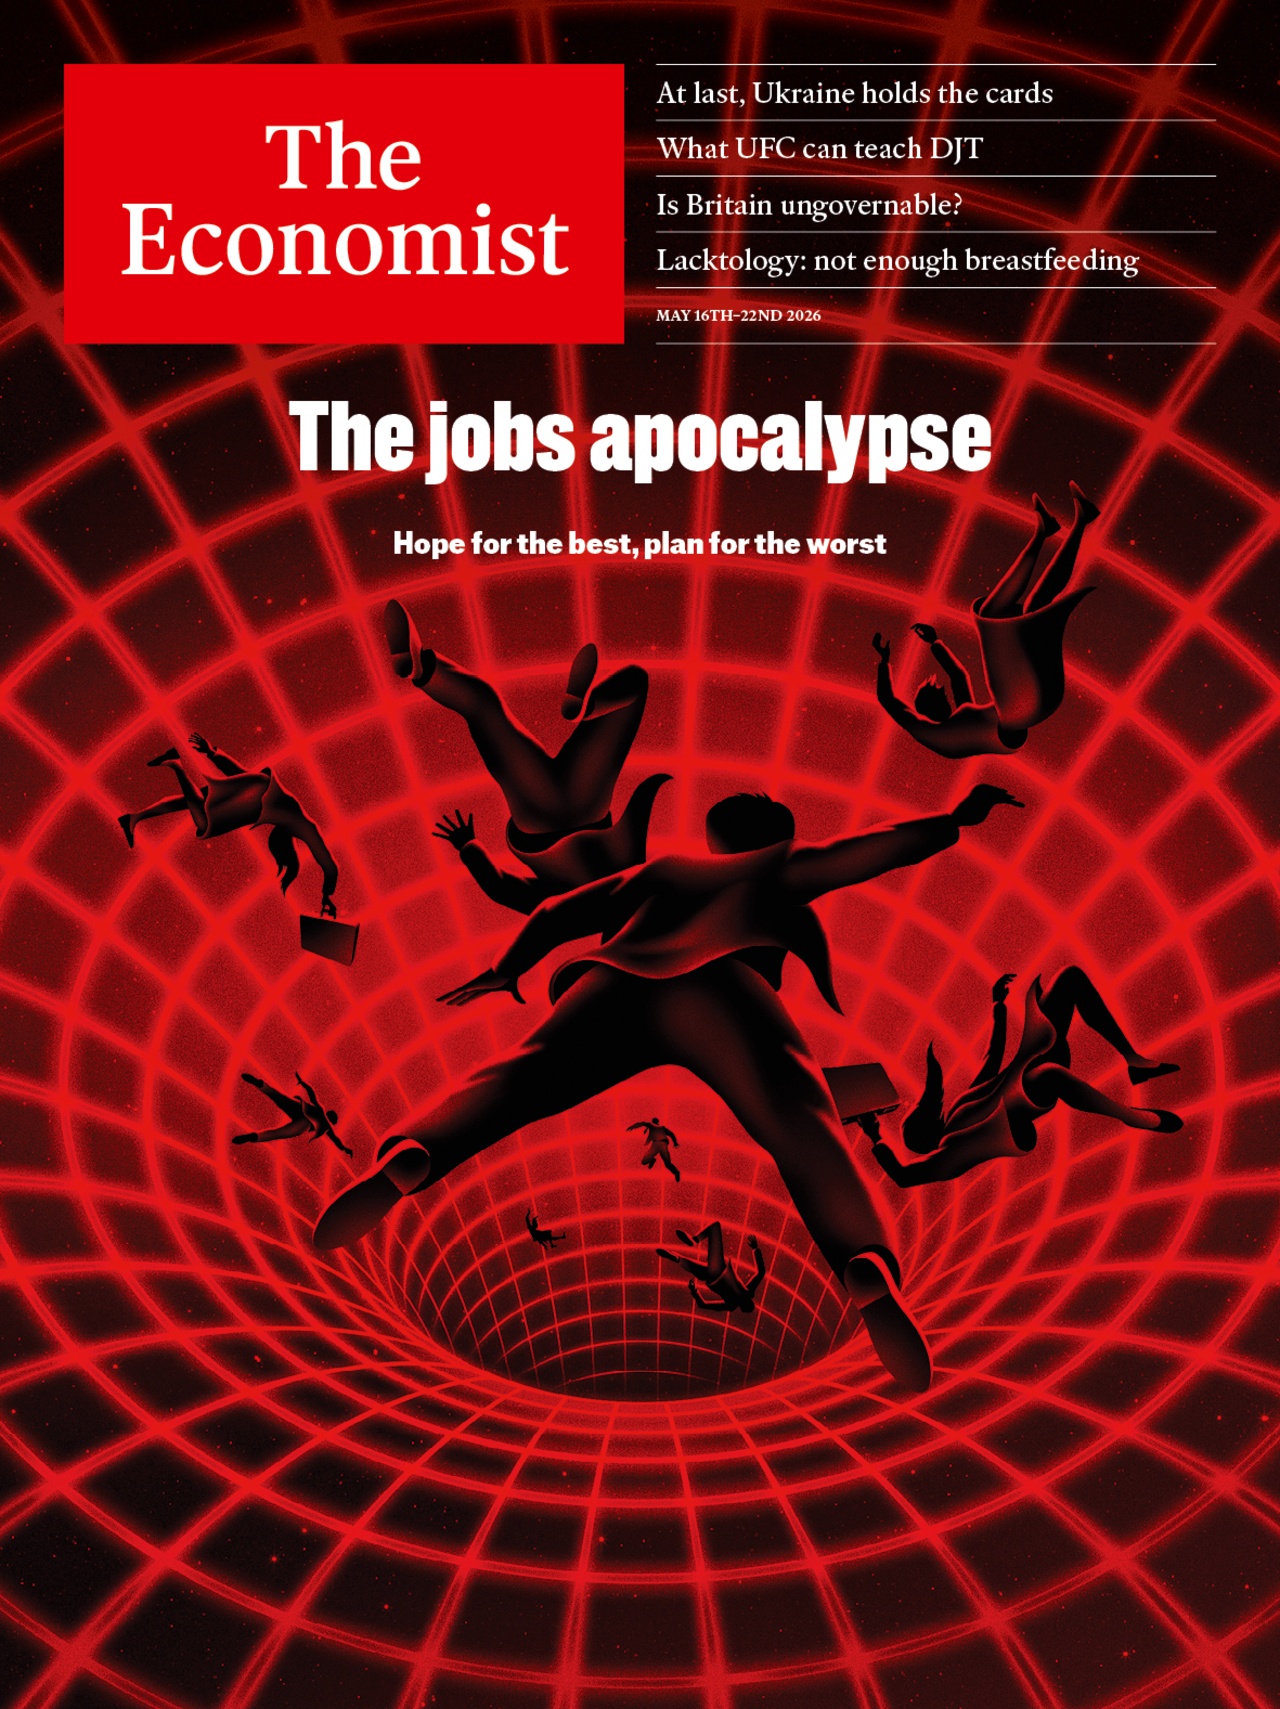
\includegraphics[height=5cm,keepaspectratio]{Economist_jobs_apocalypse.jpg}};
  \node<2->[rotate=3]  at (0, -0.3) {%
    \includegraphics[height=5cm,keepaspectratio]{{Atlantic_AI Has Ruined the Job Market}.JPG}};
  \node<3->[rotate=-2] at (4, 0.2) {%
    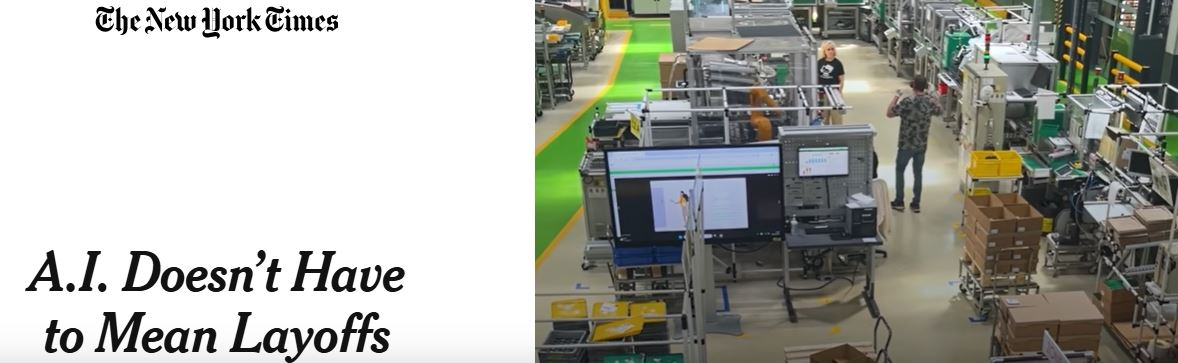
\includegraphics[height=5cm,keepaspectratio]{NYTimes_AIdoesnthavetomeanlayoffs.JPG}};
\end{tikzpicture}

\vspace{0.4em}
\end{frame}

% ---------------------------------------------------------------
\begin{frame}{Recent literature: AI exposure and employment}
\footnotesize
\setlength{\tabcolsep}{4pt}
\begin{tabular}{l l p{6.8cm}}
\toprule
Country & Paper & Headline (youngest workers, top quintile) \\
\midrule
United States  & Brynjolfsson, Chandar \& Chen (2025) & Q5 ages 22--25 decline $\sim 16$ log pts \\
Sweden         & Lodefalk et al.\ (2026)              & Q5 ages 22--25 decline $\sim 5.5\,\%$; monotonic gradient \\
United Kingdom & Teeselink (2025)                     & $-0.3\%$ per SD LLM (large language model) exposure; concentrated in junior, high-wage \\
39 countries   & Teeselink (2026)                     & Hiring declines; sharper under strict employment protection legislation \\
Denmark        & Humlum \& Vestergaard (2026)         & Null at firm level: workplace adoption rules out effects $> 1/3$ ppt on early-career share \\
Finland        & Kauhanen et al.\ (2024, 2025, 2026)  & Null; demographic explanation \\
\bottomrule
\end{tabular}

\vspace{0.8em}
\end{frame}

% ---------------------------------------------------------------
\begin{frame}{Contributions}
\begin{itemize}\setlength{\itemsep}{8pt}
  \item Complement the international literature on AI exposure and employment pre/post ChatGPT with results on Norway  
  \item Study the recent impact of \textbf{Agentic AI} ( \emph{``autonomous LLM-based systems that plan, use tools, and execute multi-step research tasks''} (Korinek, 2025)) 
  \item Track developments of the universe of Norwegian employment ``live'' 
\end{itemize}
\end{frame}


% ---------------------------------------------------------------
\section{Data}
% Data and methodology

\begin{frame}{Data: A-ordningen}
\begin{itemize}\setlength{\itemsep}{6pt}
  \item Norway's mandatory employer-reporting system; universe of formal employment.
  \item Coverage: $\sim 3.1$ million workers per month, January 2021 through February 2026.
  \item Variables used: 4-digit STYRK-08 occupation, age (monthly precision), institutional sector, cash earnings (\emph{kontantlønn}), position percentage, contracted hours, new-job flag.
  \item Two analysis units:
  \begin{itemize}
    \item \textbf{Cell counts and means} (occupation $\times$ age $\times$ month $\times$ sector) for the descriptive series.
    \item \textbf{Individual records} (firm $\times$ age $\times$ occupation $\times$ month) for the firm-FE design.
  \end{itemize}
  \item Index date: October 2022 = 1, the month before ChatGPT's public release.
\end{itemize}
\end{frame}

% ---------------------------------------------------------------
\begin{frame}{Constructing exposure quintiles}
\begin{itemize}\setlength{\itemsep}{8pt}
  \item Rank the 397 STYRK-08 codes that the Eloundou et al.\ mapping covers by $\beta$.
  \item Assign each 4-digit code to one of five quintiles on the \emph{occupation} distribution.
  \item Each code counts once, regardless of its employment share.
  \item Quintile assignment is fixed throughout the period.
\end{itemize}
\end{frame}


% ---------------------------------------------------------------
%\section{Why Eloundou}
% Why we use Eloundou (with hyperlink to LORV Fig 1 backup slide)

\begin{frame}{Focus on exposure measure of Eloundou et al.}
\hypertarget{after-eloundou}{}
\begin{itemize}\setlength{\itemsep}{10pt}
  \item \textbf{Commonly used, standard measure.} Published in \textit{Science} (2024), used by Brynjolfsson, Chandar \& Chen (2025), later by Teeselink (2025), Humlum \& Vestergaard (2026), Kauhanen \& Rouvinen (2026), Lodefalk et al.\ (2026).
  \item \textbf{Best validation against observed AI use.} In Lindenlaub, Oh, Rodríguez \& Veldkamp (2026, Fig.\ 1), Eloundou et al.\ has $R^2 = 0.30$ against worker-reported adoption, ahead of Handa (0.26), Felten (0.26), and Webb (0.02).
\end{itemize}

\vspace{1.2em}
\hfill\hyperlink{lorv-detail}{\beamerbutton{Show Lindenlaub et al.\ Fig.\ 1}}
\end{frame}


% ---------------------------------------------------------------
%\section{Mapping AI exposure to STYRK-08}
% Mapping section: reuse Eloundou-only material from slides/mapping/.
% Core frames only in the main flow; the worked examples, the task-level
% scoring tables, the many-to-one example and the O*NET intro live in the
% Backup section (90_backup.tex).

% Brief intro: why a mapping is needed
\begin{frame}{Mapping from US to Norwegian occupation codes}
\begin{itemize}\setlength{\itemsep}{8pt}
  \item Eloundou et al.'s exposure measure is built on US occupation codes (SOC).
  \item Norwegian register data use STYRK-08.
  \item STYRK-08 is based on ISCO-08; overlapping 4-digit unit groups are code-compatible after a small set of documented Norwegian-title checks.
  \item Bridge: SOC $\to$ ISCO-08 via US Bureau of Labor Statistics (BLS), then match overlapping STYRK-08 codes with manual SOC-source corrections for 2267 and 2269.
\end{itemize}
\end{frame}

% Eloundou concept, chain, pharmacists worked example
% Eloundou et al. (2024): task-level LLM exposure -- core frames
% (split out of eloundou.tex so the presentation deck can input only these)

\begin{frame}{What Eloundou et al.\ measure}
\begin{itemize}\setlength{\itemsep}{6pt}
  \item Each O*NET task rated by humans and GPT-4 on three categories:
  \begin{itemize}
    \item[$E_0$] no exposure
    \item[$E_1$] LLM alone reduces task time by $\geq 50\%$
    \item[$E_2$] LLM with complementary software reduces task time by $\geq 50\%$
  \end{itemize}
  \item Task-level score:\quad
        $\beta_{\text{task}} = 0$ if $E_0$,\;\; $1$ if $E_1$,\;\; $0.5$ if $E_2$
  \item Occupation score: $\beta_{\text{occ}}$ = mean of $\beta_{\text{task}}$ with O*NET Core tasks weighted 2, Supplemental tasks 1
  \item We use the published occupation-level file (\texttt{occ\_level.csv}); it differs slightly from unweighted task means where an occupation has Supplemental tasks
\end{itemize}
\end{frame}

% ---------------------------------------------------------------
\begin{frame}{The code chain}
\centering
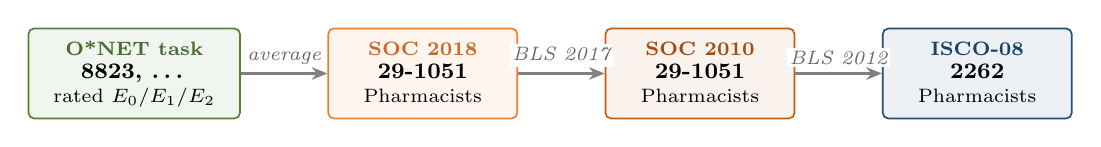
\begin{tikzpicture}[node distance=1.0cm and 1.1cm]
  \node[codebox=cTASK] (task) {\cbox{cTASK}{O*NET task}{8823, \dots}{rated $E_0/E_1/E_2$}};
  \node[codebox=cSOC18, right=of task] (soc18) {\cbox{cSOC18}{SOC 2018}{29-1051}{Pharmacists}};
  \node[codebox=cSOC10, right=of soc18] (soc10) {\cbox{cSOC10}{SOC 2010}{29-1051}{Pharmacists}};
  \node[codebox=cSTYRK, right=of soc10] (isco) {\cbox{cSTYRK}{ISCO-08}{2262}{Pharmacists}};

  \draw[chain] (task) -- node[arrowlabel]{average} (soc18);
  \draw[chain] (soc18) -- node[arrowlabel]{BLS 2017} (soc10);
  \draw[chain] (soc10) -- node[arrowlabel]{BLS 2012} (isco);
\end{tikzpicture}

\vspace{1em}
Overlapping 4-digit unit groups in STYRK-08 are code-compatible with ISCO-08 (SSB Notater 17/2011). STYRK 2262 is Farmasøyter.
\end{frame}

% ---------------------------------------------------------------
\begin{frame}{Worked example: Pharmacists (one-to-one mapping)}
\centering
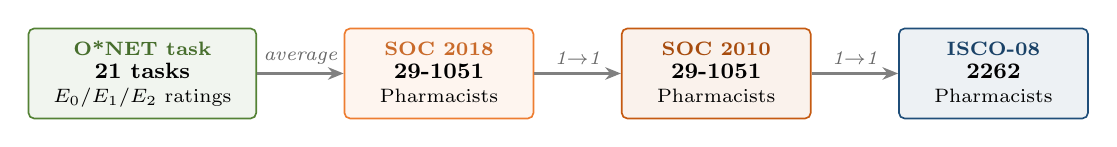
\begin{tikzpicture}[node distance=1.0cm and 1.1cm]
  \node[codebox=cTASK] (task) {\cbox{cTASK}{O*NET task}{21 tasks}{$E_0/E_1/E_2$ ratings}};
  \node[codebox=cSOC18, right=of task] (soc18) {\cbox{cSOC18}{SOC 2018}{29-1051}{Pharmacists}};
  \node[codebox=cSOC10, right=of soc18] (soc10) {\cbox{cSOC10}{SOC 2010}{29-1051}{Pharmacists}};
  \node[codebox=cSTYRK, right=of soc10] (isco) {\cbox{cSTYRK}{ISCO-08}{2262}{Pharmacists}};

  \draw[chain] (task) -- node[arrowlabel]{average} (soc18);
  \draw[chain] (soc18) -- node[arrowlabel]{1$\to$1} (soc10);
  \draw[chain] (soc10) -- node[arrowlabel]{1$\to$1} (isco);
\end{tikzpicture}

\vspace{1em}
\begin{itemize}\setlength{\itemsep}{4pt}
  \item Pharmacists carry the same 6-digit SOC in both vintages: 29-1051
  \item BLS crosswalk sends 29-1051 to a single ISCO-08 code (2262)
  \item Norwegian STYRK 2262 is Farmasøyter, no Norway-specific re-coding
\end{itemize}
\end{frame}

% ---------------------------------------------------------------
\begin{frame}{Task-level scoring for Pharmacists (SOC 29-1051, all 21 tasks)}
\centering\scriptsize
\setlength{\tabcolsep}{4pt}
\renewcommand{\arraystretch}{0.95}
\begin{tabular}{p{5.5cm}cc @{\hspace{0.7cm}} p{5.5cm}cc}
\toprule
O*NET task & $E$ & $\beta$ & O*NET task & $E$ & $\beta$ \\
\midrule
\rO{Review prescriptions for accuracy}{$E_2$}{0.5}             & \rO{Refer patients to other professionals}{$E_2$}{0.5} \\
Assess identity, strength, purity of meds     & $E_0$ & 0.0 & \rO{Work in hospitals/clinics or for HMOs}{$E_2$}{0.5} \\
\rO{Provide info on drug interactions}{$E_2$}{0.5}             & \rR{Update or troubleshoot pharmacy databases}{$E_1$}{1.0} \\
\rO{Analyze prescribing trends}{$E_2$}{0.5}                    & \rO{Manage pharmacy operations, hire, supervise}{$E_2$}{0.5} \\
\rO{Maintain pharmacy files and patient profiles}{$E_2$}{0.5}  & Prepare sterile solutions                           & $E_0$ & 0.0 \\
\rO{Collaborate with other health professionals}{$E_2$}{0.5}   & Offer health promotion / prevention activities      & $E_0$ & 0.0 \\
Plan procedures for mixing and labeling       & $E_0$ & 0.0 & Assay radiopharmaceuticals                          & $E_0$ & 0.0 \\
\rO{Order and purchase pharmaceutical supplies}{$E_2$}{0.5}    & \rR{Publish educational information}{$E_1$}{1.0} \\
Compound and dispense medications             & $E_0$ & 0.0 & & & \\
\rO{Contact insurance companies on billing}{$E_2$}{0.5}        & \multicolumn{3}{l}{\textbf{Counts:} 6 $E_0$ \quad 3 $E_1$ \quad 12 $E_2$} \\
\rO{Advise customers on medication brands}{$E_2$}{0.5}         & & & \\
\rR{Teach pharmacy students serving as interns}{$E_1$}{1.0}    & \multicolumn{3}{l}{\textbf{Occupation $\beta$ (mean of 21):} \;\; \textbf{0.4286 (Q4)}} \\
\rO{Provide services for diabetes, asthma, etc.}{$E_2$}{0.5}   & & & \\
\bottomrule
\end{tabular}
\end{frame}


% Distribution across Norwegian occupations (employment-weighted)
% Eloundou β distribution across STYRK occupations (unweighted + employment-weighted)

\begin{frame}{Distribution of Eloundou et al.\ $\beta$ across Norwegian occupations}
\centering
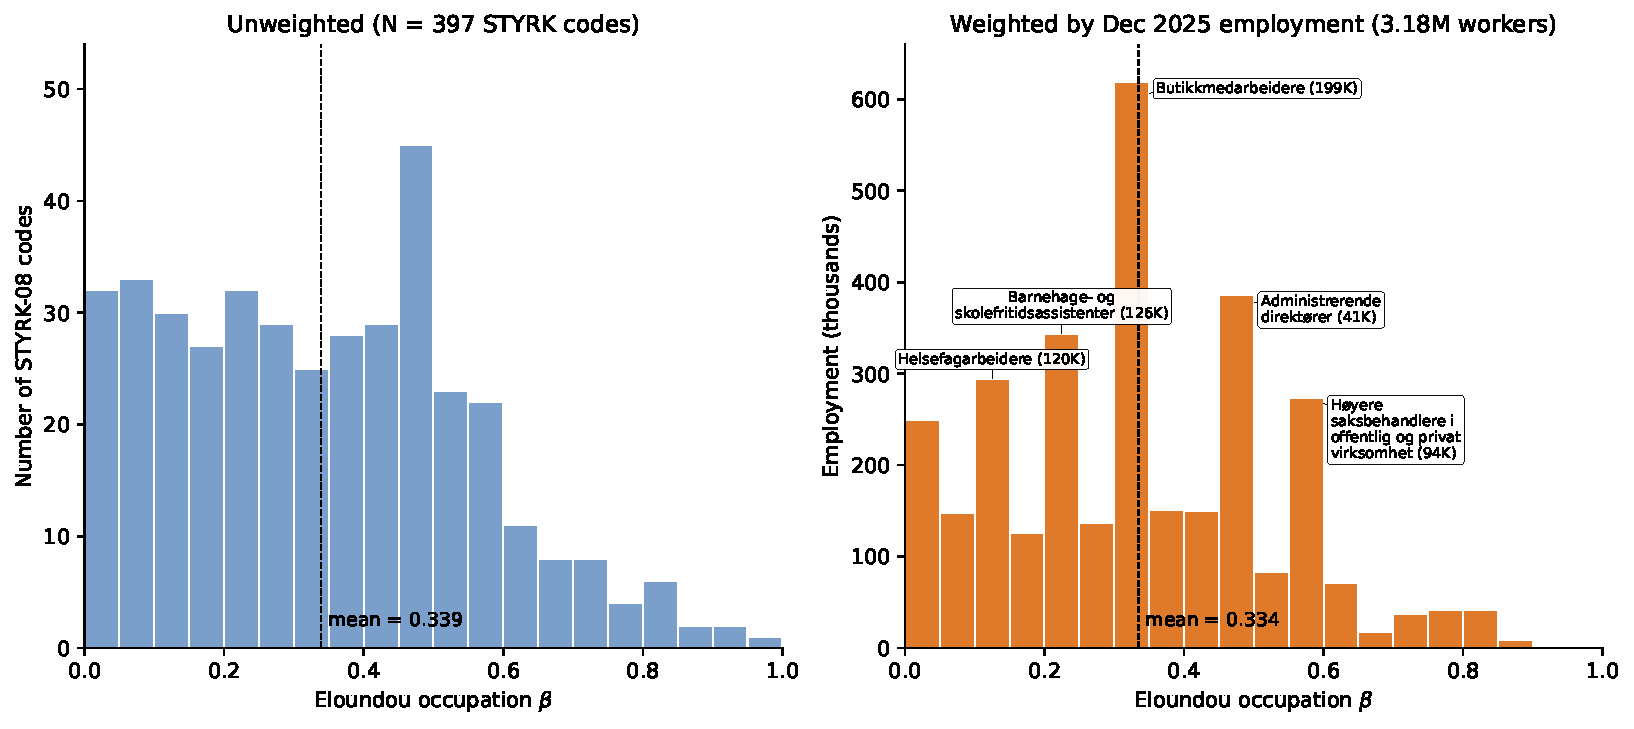
\includegraphics[width=\linewidth,height=5cm,keepaspectratio]{eloundou_distribution.pdf}

\vspace{0.3em}
\footnotesize
Left: one observation per STYRK-08 code (397 codes; mean 0.34). Right: the same distribution weighted by December 2025 employment (3.18M workers; mean 0.33); the largest single occupations are labelled. Large occupations sit across the whole exposure range, from health care workers (0.11) to policy administration professionals (0.57).
\end{frame}


% ---------------------------------------------------------------
\begin{frame}{Five largest occupations per exposure quintile (Apr 2026)}
\hypertarget{after-mapping}{}
\begin{columns}[T,onlytextwidth]
\begin{column}{0.50\textwidth}
\scriptsize
\setlength{\tabcolsep}{3pt}
\renewcommand{\arraystretch}{0.92}
\begin{tabular}{@{}p{4.6cm} r r@{}}
\toprule
Occupation & Score & Emp. \\
\midrule
\multicolumn{3}{@{}l}{\textit{Q1 (least exposed)}} \\
Cleaners (offices, hotels, \ldots) & 0.03 & 40k \\
Building electricians & 0.13 & 26k \\
Food machine operators & 0.09 & 23k \\
Motor vehicle mechanics & 0.09 & 17k \\
Plumbers and pipe fitters & 0.06 & 17k \\
\addlinespace
\multicolumn{3}{@{}l}{\textit{Q2}} \\
Carpenters and joiners & 0.14 & 35k \\
Child care workers & 0.25 & 32k \\
Waiters & 0.16 & 20k \\
Machinery mechanics and repairers & 0.13 & 16k \\
Cooks & 0.19 & 16k \\
\addlinespace
\multicolumn{3}{@{}l}{\textit{Q3}} \\
Shop sales assistants & 0.34 & 115k \\
Stock clerks & 0.33 & 29k \\
Heavy truck and lorry drivers & 0.31 & 21k \\
Science technicians (n.e.c.) & 0.36 & 20k \\
Car, taxi and van drivers & 0.28 & 14k \\
\bottomrule
\end{tabular}
\end{column}
\begin{column}{0.50\textwidth}
\scriptsize
\setlength{\tabcolsep}{3pt}
\renewcommand{\arraystretch}{0.92}
\begin{tabular}{@{}p{4.6cm} r r@{}}
\toprule
Occupation & Score & Emp. \\
\midrule
\multicolumn{3}{@{}l}{\textit{Q4}} \\
Retail/wholesale trade managers & 0.48 & 30k \\
Managing directors / CEOs & 0.49 & 28k \\
Civil engineers & 0.48 & 19k \\
Sales and marketing managers & 0.48 & 13k \\
Construction managers & 0.44 & 12k \\
\addlinespace
\multicolumn{3}{@{}l}{\textit{Q5 (most exposed)}} \\
Commercial sales representatives & 0.57 & 37k \\
General office clerks & 0.60 & 33k \\
Systems analysts & 0.63 & 22k \\
Software developers (n.e.c.) & 0.77 & 18k \\
Accounting associate profs.\ & 0.80 & 15k \\
\bottomrule
\end{tabular}

\vspace{0.6em}
\footnotesize Employment in thousands. Private sector, ages 21--60, ranked within quintile by April 2026 headcount.

\vspace{0.3em}
\hfill\hyperlink{worked-examples}{\beamerbutton{More worked examples}}
\end{column}
\end{columns}
\end{frame}


% ---------------------------------------------------------------
\section{Employment gaps by AI exposure}
% Descriptive results

\begin{frame}{All ages pooled: the most exposed do not pull away}
\centering
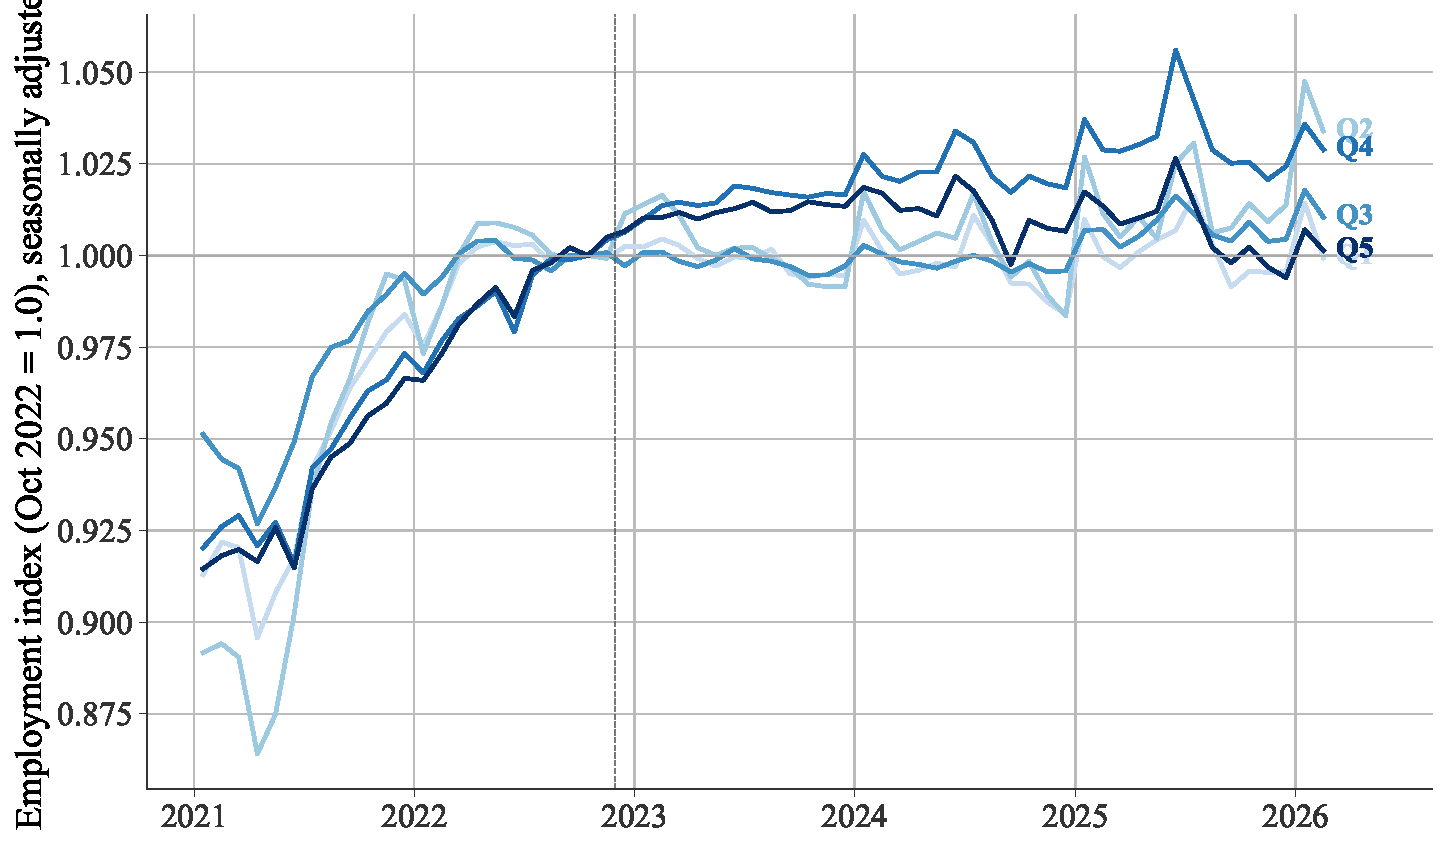
\includegraphics[height=5.8cm,keepaspectratio]{figure_emp_byexposure_sa.pdf}

\vspace{0.2em}
\footnotesize
Ages 21--60, private sector, seasonally adjusted, indexed to October 2022 = 1. Q5 (most exposed) tracks Q1 (least exposed) throughout. The paper analog of the kiindeksen.no headline figure.
\end{frame}

% ---------------------------------------------------------------
\begin{frame}{Case studies: the canary pattern is real}
\centering
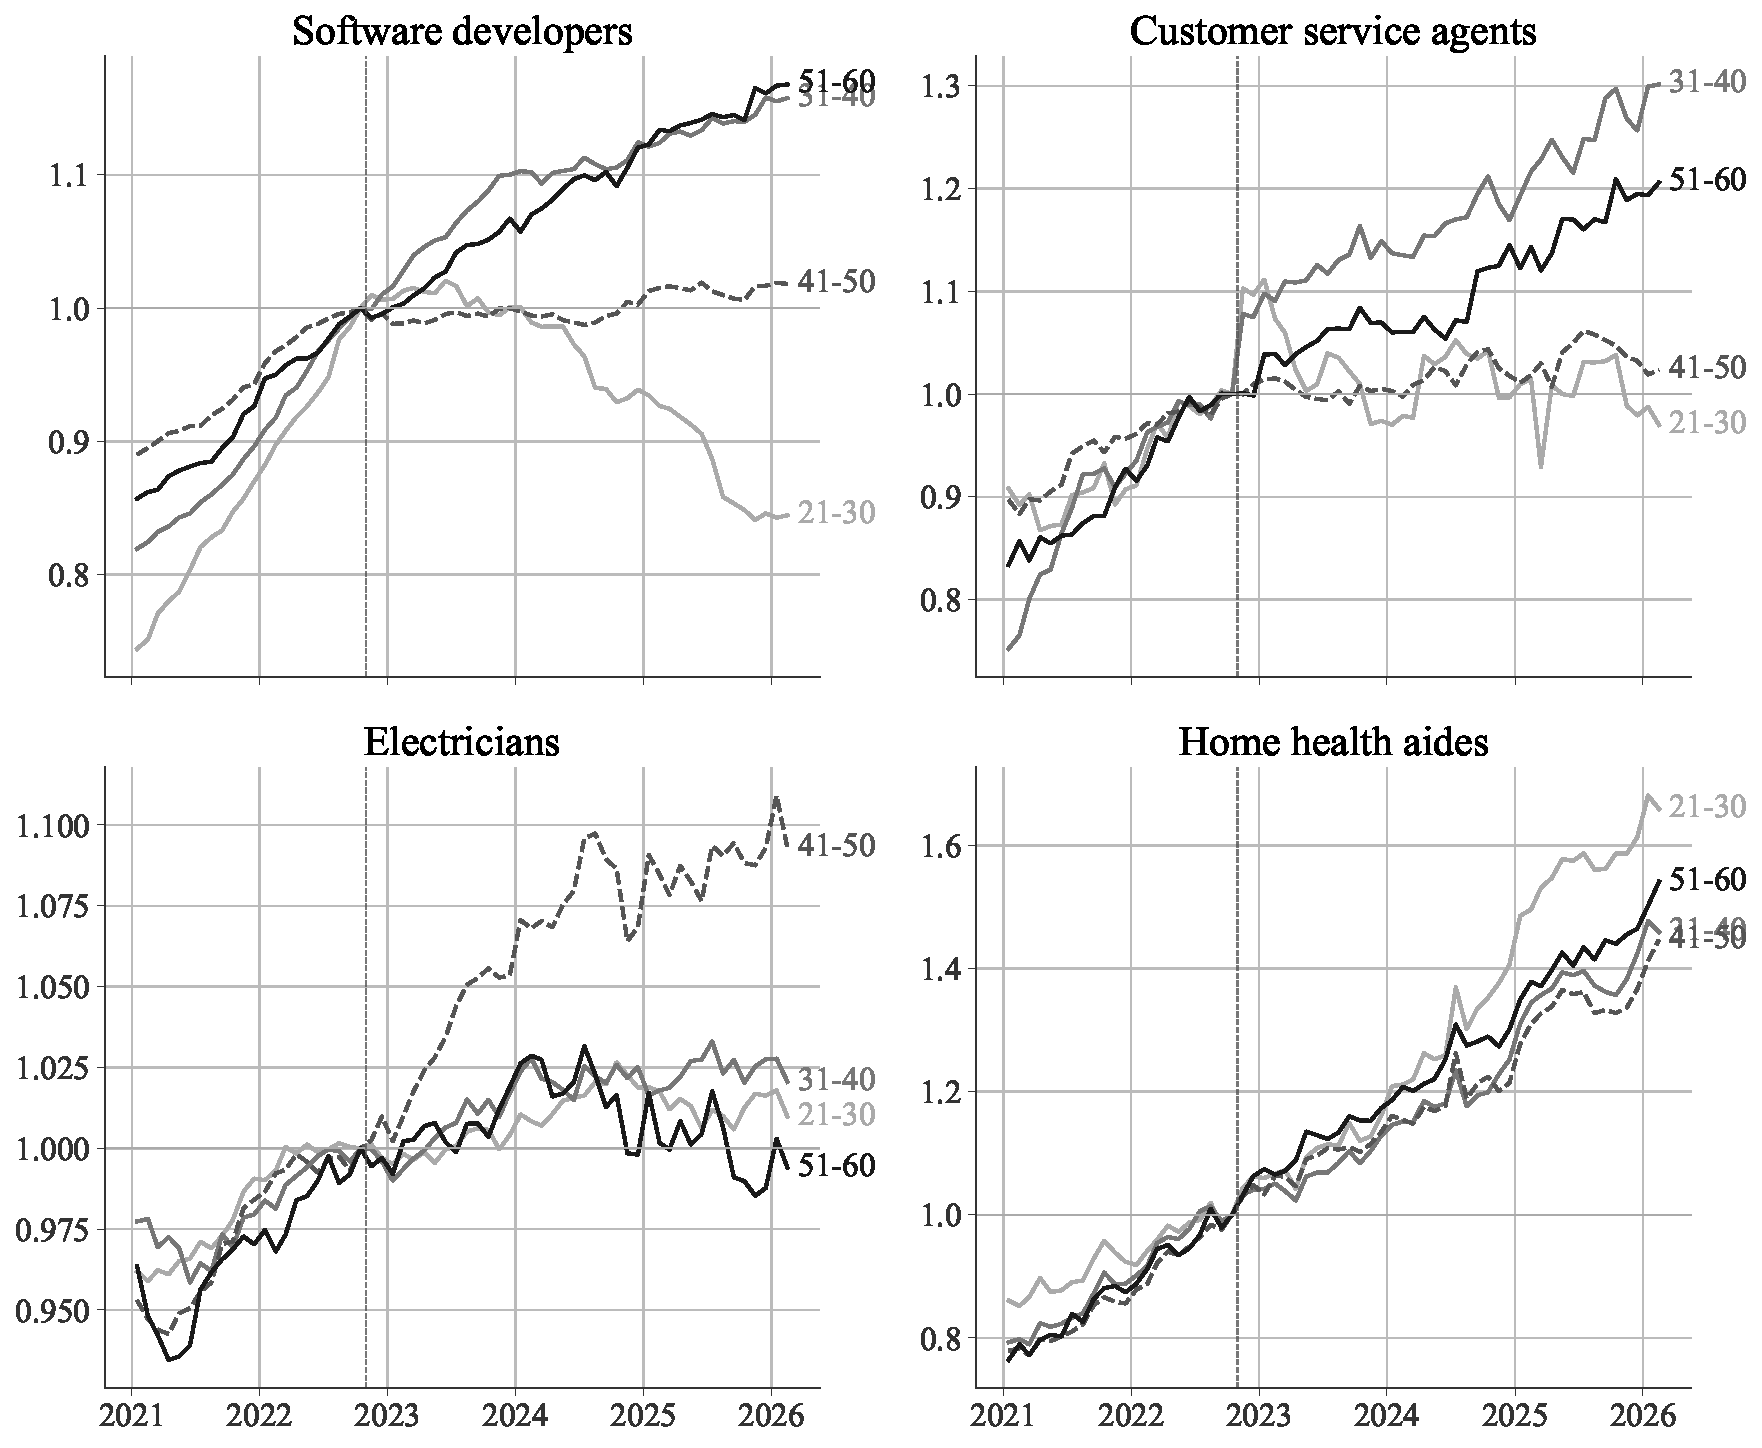
\includegraphics[height=5.6cm,keepaspectratio]{figure_occupations_by_age_sa.pdf}

\vspace{0.2em}
\footnotesize
Software developers aged 21--30 decline sharply after ChatGPT ($\sim -18\,\%$ per capita); customer service agents show the same shape, milder. Electricians and home health aides, the low-exposure benchmarks, do not.
\end{frame}

% ---------------------------------------------------------------
\begin{frame}{Private sector: employment by exposure quintile and age}
\hypertarget{after-private}{}
\centering
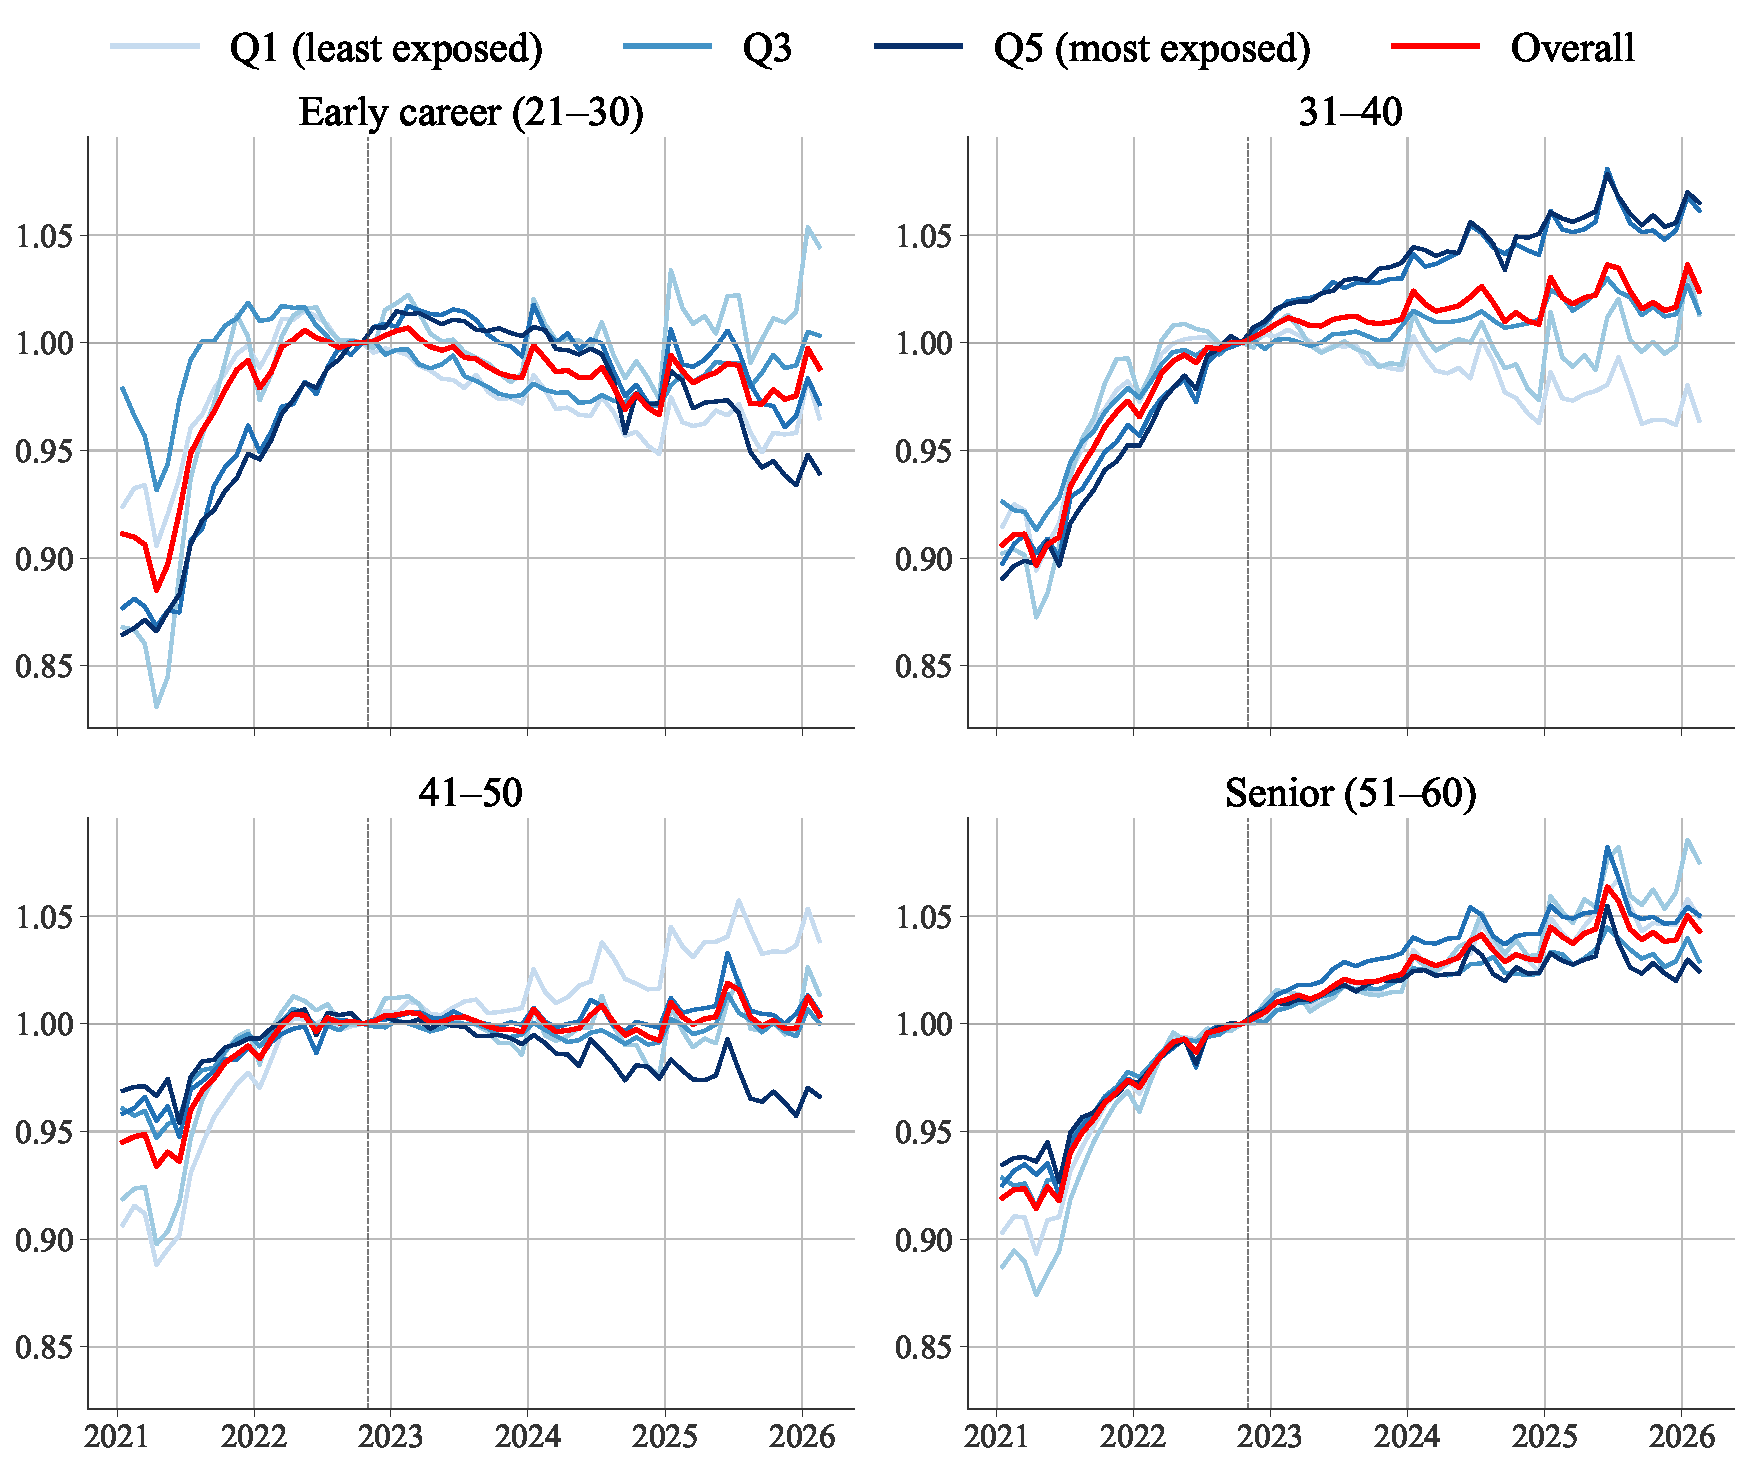
\includegraphics[height=5.6cm,keepaspectratio]{figure_emp_decade_private_sa.pdf}

\vspace{0.2em}
\footnotesize
Seasonally adjusted. No clear pattern of Q5 losing ground among the youngest: at 21--30, Q5 drifts a few points below Q1 from mid-2025, but the gap is smaller than pre-period swings.

\vspace{-0.2em}
\hfill\hyperlink{public-sector-detail}{\beamerbutton{Public sector}}\;\hyperlink{cash-earnings-detail}{\beamerbutton{Cash earnings}}
\end{frame}

% ---------------------------------------------------------------
\begin{frame}{Automation vs.\ augmentation (Handa et al.)}
\hypertarget{after-handa}{}
\centering
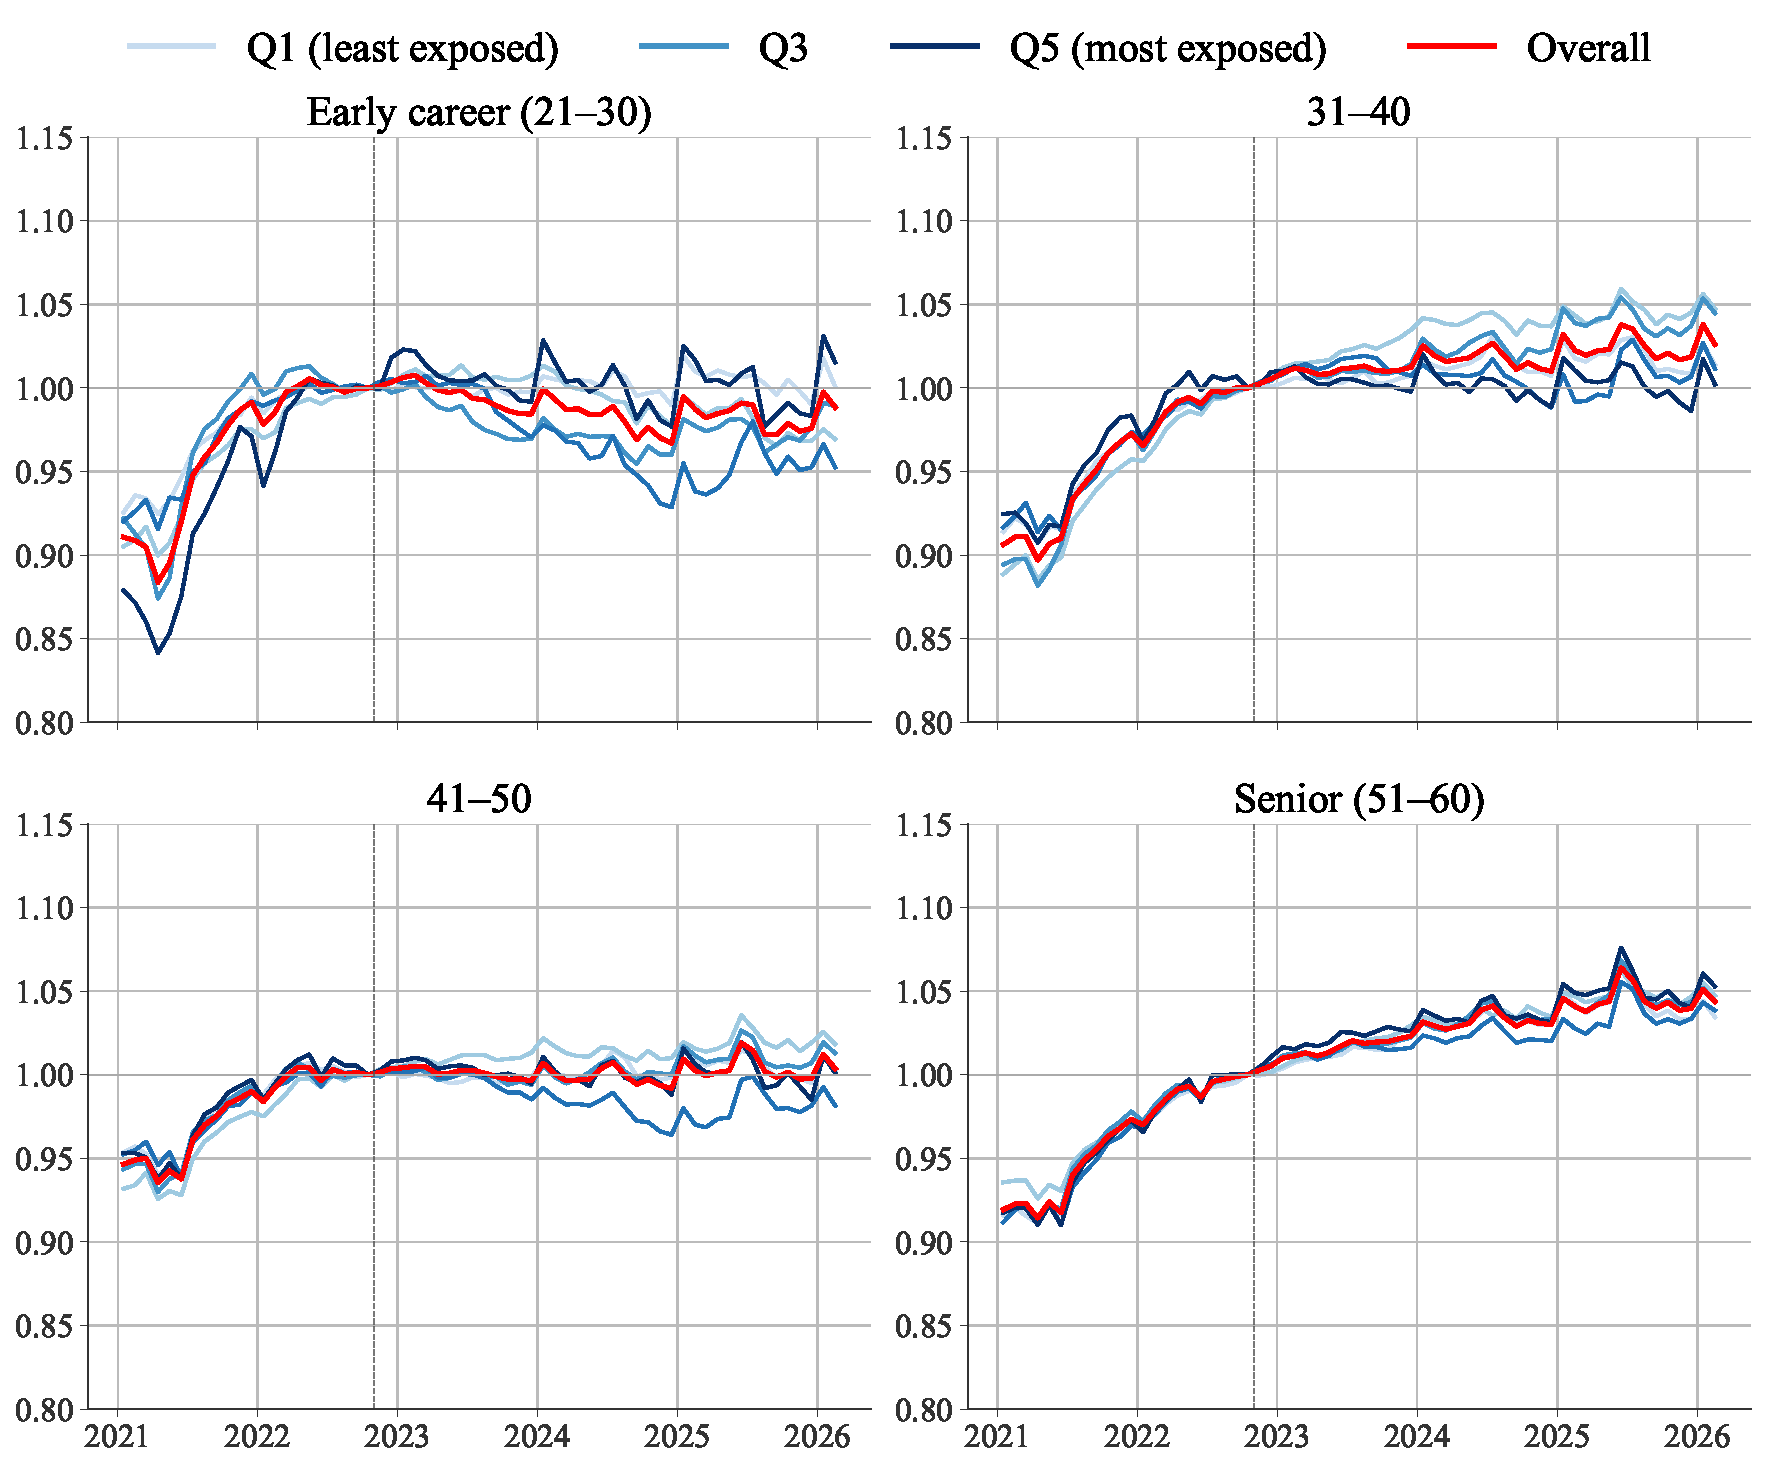
\includegraphics[height=5.6cm,keepaspectratio]{figure_age_by_quintile_handa_auto_sa.pdf}

\vspace{0.2em}
\footnotesize
Quintiles ranked by \textbf{automation} share of Claude usage. Among the two youngest groups, the most-exposed quintile declines relative to the least exposed, more visibly from late 2025. The augmentation ranking shows no such gradient.

\vspace{-0.2em}
\hfill\hyperlink{handa-aug-detail}{\beamerbutton{Augmentation}}
\end{frame}


% ---------------------------------------------------------------
\section{Regression analysis}
% Cell-level Poisson DiD: spec + event-study results + HonestDiD
% (also hosts the METR-capability frame and the agentic re-anchor)

\begin{frame}{Empirical specification}
\begin{itemize}\setlength{\itemsep}{4pt}
  \item Cells: (occupation $j$ $\times$ age group $a$ $\times$ month $t$), private sector, 2021m1--2026m4
  \item One Poisson PPML regression per decade age group:
\end{itemize}
\[
\log E[\text{count}_{j,a,t}] = \alpha_{j} + \beta_{t} + \gamma_{q(j),\,k(t)}
\]
\begin{itemize}\setlength{\itemsep}{3pt}
  \item $\alpha_j$: occupation FE, absorbs permanent occupation size
  \item $\beta_t$: month FE, absorbs the aggregate age-cohort time path
  \item $\gamma_{q,k}$: log-point change for quintile $q$ at event time $k$, relative to \textbf{Q1} (least exposed) and $k = -1$ (October 2022)
  \item SE clustered at occupation
\end{itemize}

\vspace{0.2em}
\footnotesize
\textbf{Why Poisson?} Counts with some zeros; $\log(0+x)$ biased.\quad
Q3 (median) reference in backup.\quad\hyperlink{cell-es-q3-detail}{\beamerbutton{Q3 reference}}
\end{frame}

% ---------------------------------------------------------------
\begin{frame}{Cell-level event-study grid (Q1 reference)}
\hypertarget{after-cell-did}{}
\centering
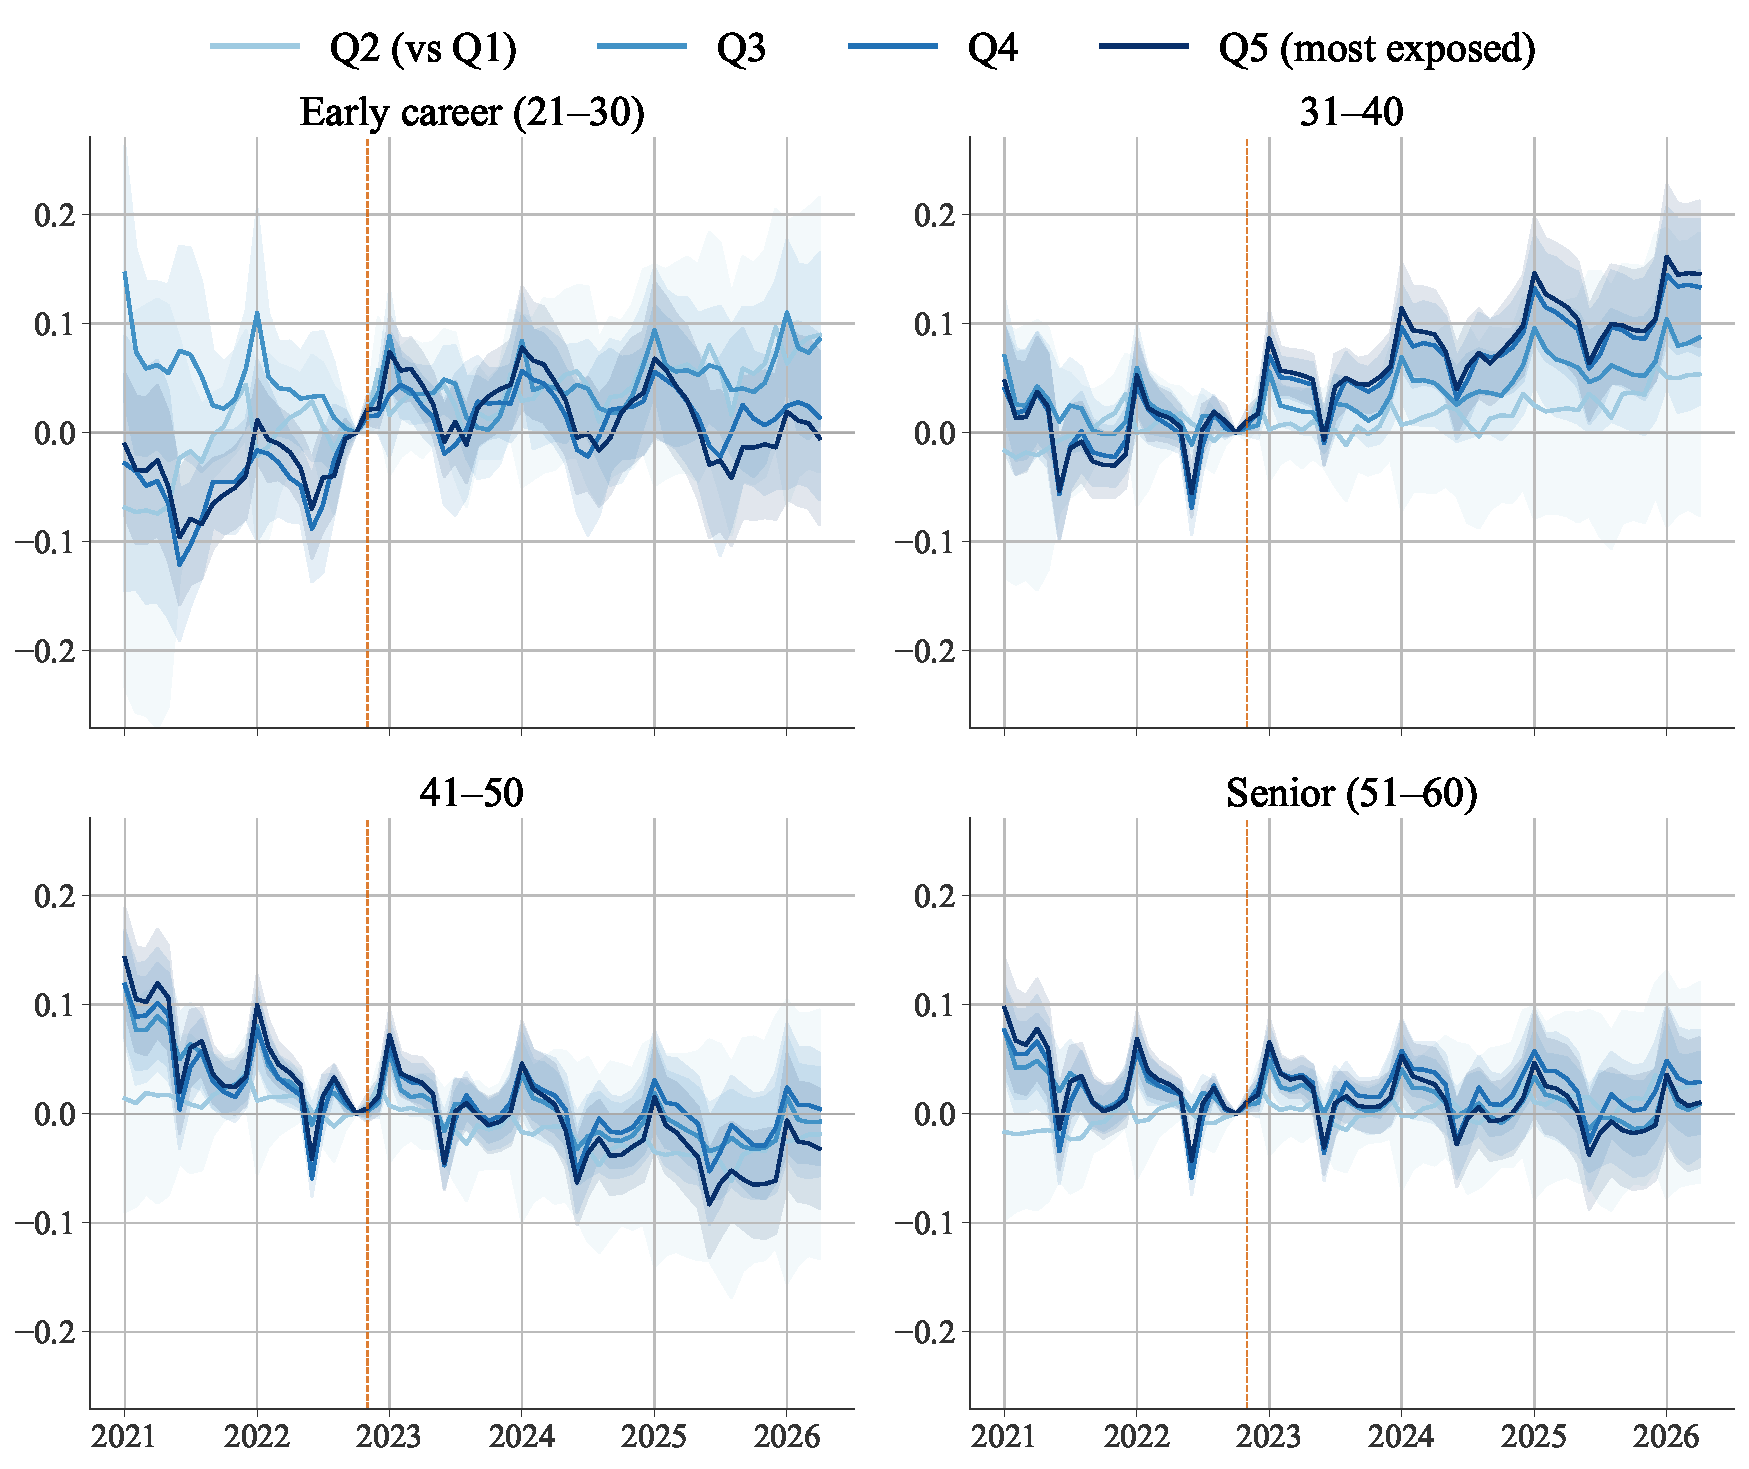
\includegraphics[height=5.6cm,keepaspectratio]{figure_microdata_poisson_es_grid.pdf}

\vspace{0.2em}
\footnotesize
Q2--Q5 vs.\ Q1, by decade age group, private sector; reference October 2022 ($k=-1$). At 21--30, Q5 is noisy and ends near zero; 31--40 rises to about $+0.15$; 41--50 reaches about $-0.08$ by mid-2025 and ends near $-0.03$; 51--60 stays near zero.
\end{frame}

% ---------------------------------------------------------------
\begin{frame}{Difference-in-differences: Q5 vs.\ Q1, post-ChatGPT average}
\centering
\setlength{\tabcolsep}{8pt}
\begin{tabular}{lcccc}
\toprule
 & 21--30 & 31--40 & 41--50 & 51--60 \\
\midrule
Q5 $\times$ Post & 0.020 & 0.081*** & $-0.015$ & 0.010 \\
                 & (0.023) & (0.019) & (0.017) & (0.017) \\
\midrule
Occupations & 391 & 393 & 393 & 392 \\
\bottomrule
\end{tabular}

\vspace{0.8em}
\begin{itemize}\setlength{\itemsep}{4pt}
  \item Stacked triple difference, Q5 $\times$ Post $\times$ young (21--30 vs.\ 31--60): $-0.009$ (0.016), n.s.
  \item No larger post-ChatGPT decline for young workers in the most exposed quintile.
\end{itemize}

\vspace{0.2em}
\footnotesize
Poisson, occupation and month FE, SE clustered at occupation. *** $p<0.01$.
\end{frame}

% ---------------------------------------------------------------
\begin{frame}{Pre-trends are not parallel. How much does it matter?}
\small
\begin{itemize}\setlength{\itemsep}{2pt}
  \item Joint tests reject parallel pre-trends in every age group; the Q5 pre-period path moves 0.11 to 0.18 log points, as large as the post-2022 movements.
  \item HonestDiD (Rambachan \& Roth 2023): post-period average Q5 vs.\ Q1, ages 21--30.
\end{itemize}

\vspace{0.2em}
\centering
\footnotesize
\renewcommand{\arraystretch}{0.95}
\begin{tabular}{lc}
\toprule
Restriction & Robust 95\% CI \\
\midrule
Original ($\bar{M}=0$, parallel trends) & [-0.022, +0.065] \\
$\bar{M}=0.5$ & [-0.221, +0.301] \\
$\bar{M}=1.0$ & [-0.475, +0.555] \\
$\bar{M}=1.5$ & [-0.729, +0.796] \\
$\bar{M}=2.0$ & [-0.983, +1.064] \\
\midrule
Breakdown $\bar{M}$ & 0.00 \\
\bottomrule
\end{tabular}


\vspace{0.3em}
The conventional interval already includes zero, so there is no gradient to overturn (breakdown $\bar M = 0$). But the null is tight only under parallel trends: the robust intervals do not rule out large effects in either direction.
\end{frame}

% ---------------------------------------------------------------
\begin{frame}{AI capability is accelerating}
\centering
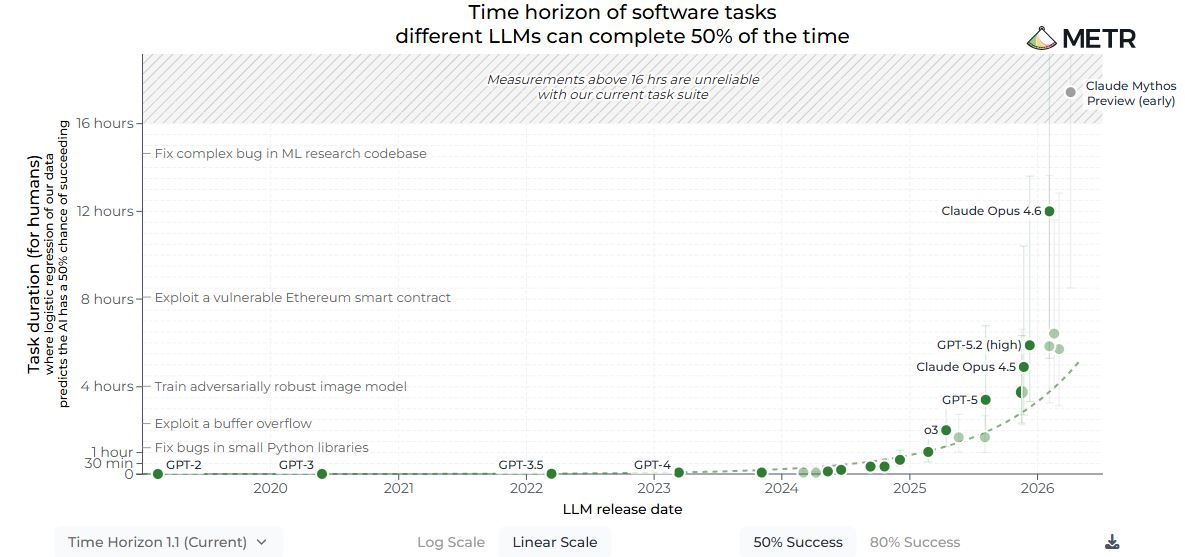
\includegraphics[height=5.5cm,keepaspectratio]{METR_time_horizon.JPG}

\vspace{0.4em}
\footnotesize
Length of software tasks an LLM completes at 50\,\% success has roughly doubled every $\sim$7 months since GPT-2. By 2026, the frontier handles multi-hour tasks. Source: Model Evaluation \& Threat Research (METR).
\end{frame}

% ---------------------------------------------------------------
\begin{frame}{Why agentic AI is a separate window}
\textbf{Mechanism.} Pre-agentic AI: AI helps with particular steps of a production chain, humans verify each step. Agentic AI: humans verify only the final output of a chain (Demirer, Horton, Immorlica \& Lucier 2026).

\vspace{0.6em}
\textbf{When did this happen?} Somewhat arbitrary, user cost falls gradually.
\begin{itemize}\setlength{\itemsep}{2pt}\footnotesize
  \item \textbf{Early 2024.} Devin demo (Mar 2024), Claude 3 Opus (Mar 2024), standardised function-calling APIs. Chaining technically possible but demo-grade.
  \item \textbf{May 2025.} OpenAI Codex (\href{https://openai.com/index/introducing-codex/}{16 May 2025}) and Anthropic Claude 4 / Claude Code (\href{https://www.anthropic.com/news/claude-4}{22 May 2025}) make multi-step coding agents production-grade.
\end{itemize}
\end{frame}

% ---------------------------------------------------------------
\begin{frame}{Re-anchor to agentic AI (April 2025)}
\centering
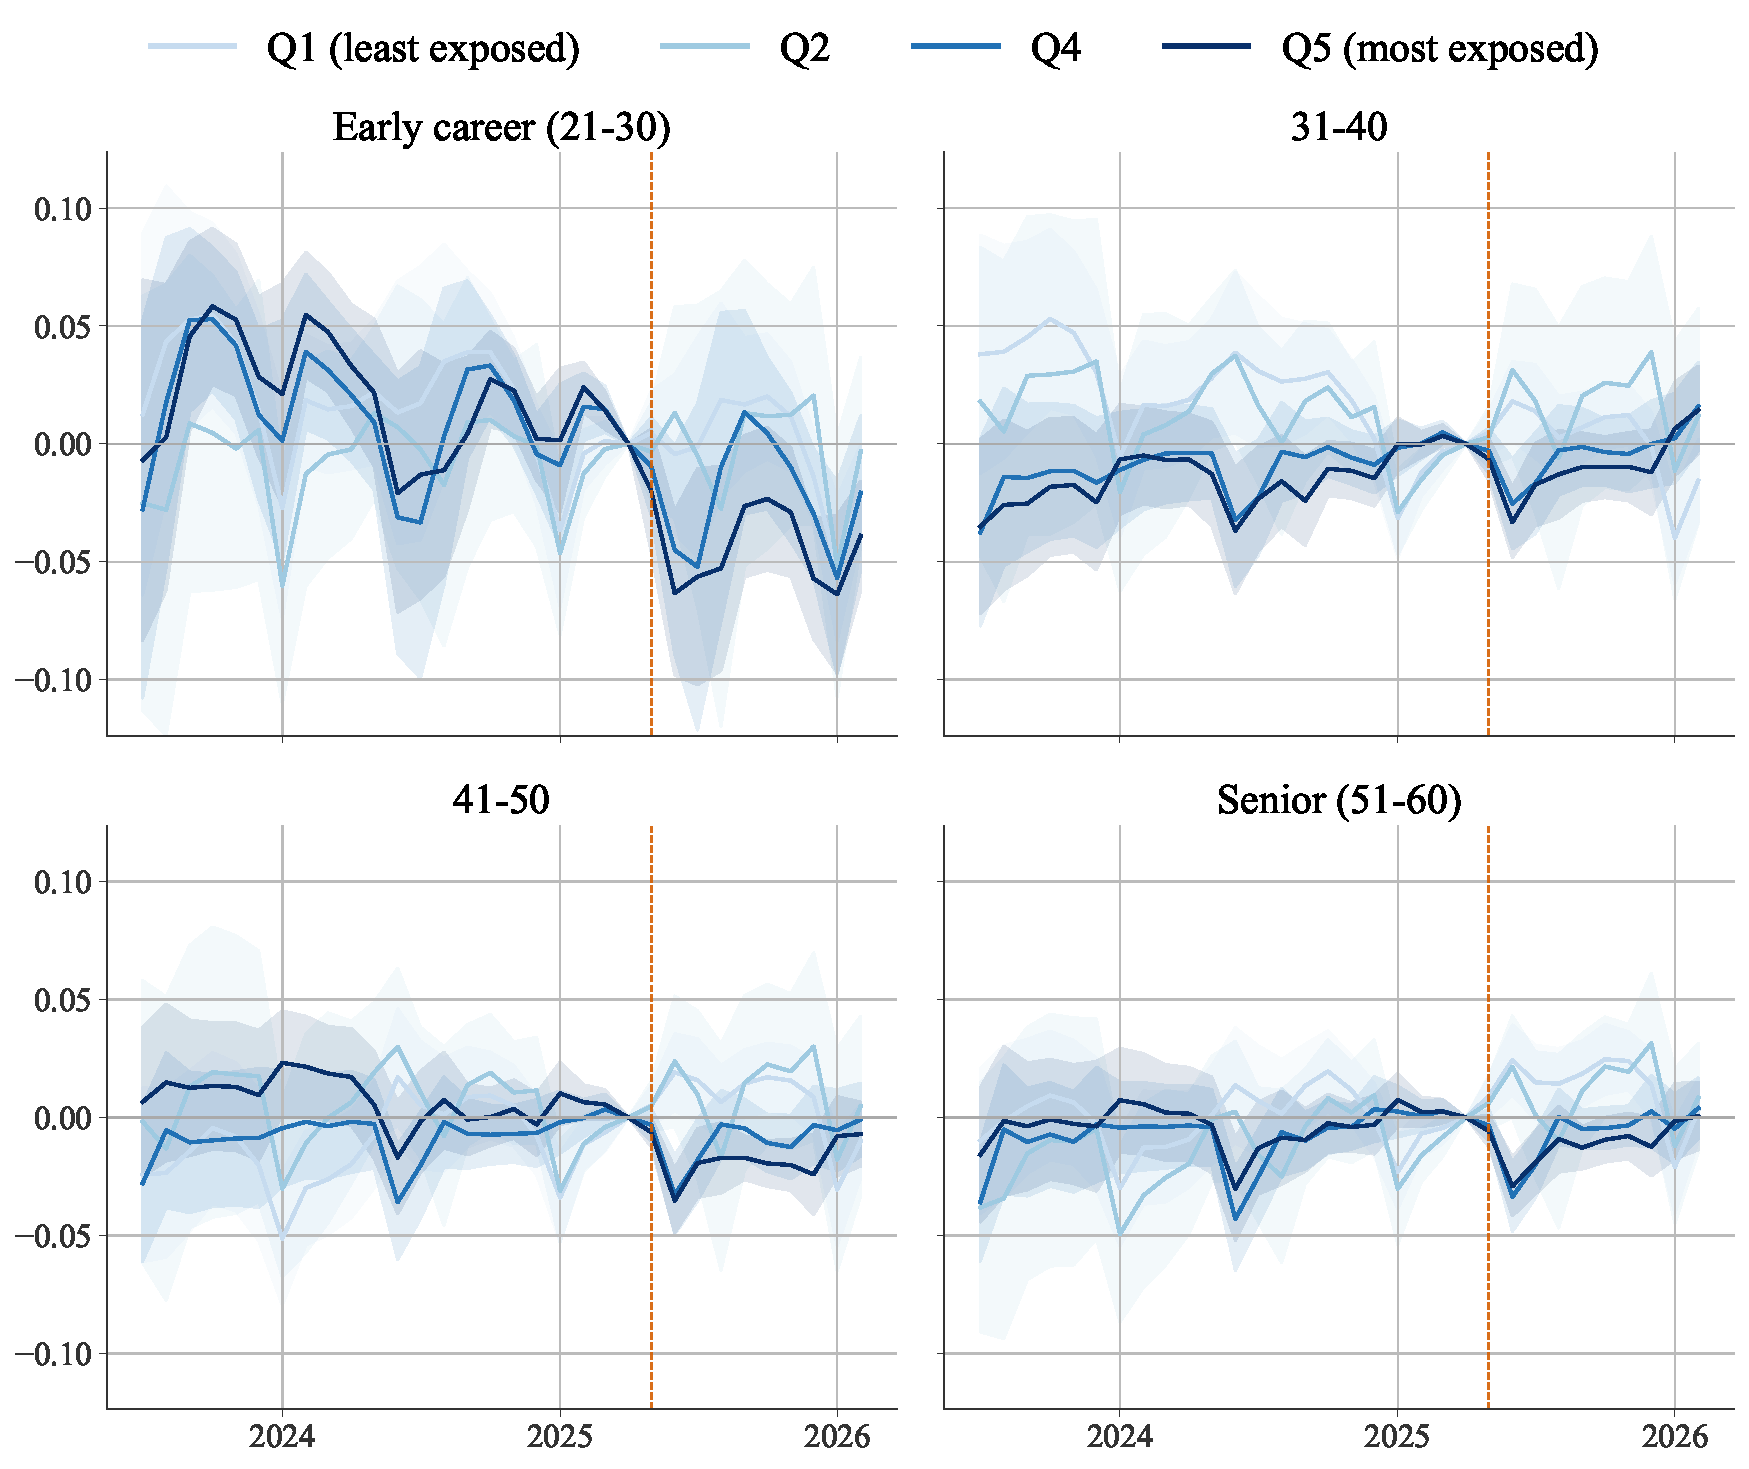
\includegraphics[height=5.6cm,keepaspectratio]{figure_microdata_es_decade_agentic.pdf}

\vspace{0.2em}
\footnotesize
Same Poisson DiD, re-anchored to April 2025 (last pre-agentic month). Pre-period 2023m1--2025m4, post 2025m5--2026m2. Cell-level, private sector. Q3 reference, estimated on data through February 2026.
\end{frame}


% ---------------------------------------------------------------
\section{Validation: individual-level data}
% Validation with individual-level data: firm fixed effects,
% cell-vs-firm reconciliation, and the BCC 22-25 replication.

\begin{frame}{Validation: within-firm reallocation}
\begin{itemize}\setlength{\itemsep}{6pt}
  \item The cell-level gradient could reflect compositional shifts across firms rather than within-firm reallocation.
  \item We re-estimate on individual-level register data with firm fixed effects, as in Brynjolfsson--Chandar--Chen.
  \item Individual-level data is a snapshot; we use it to validate the cell-level pattern, not for time-tracking.
\end{itemize}

\vspace{0.6em}
\textbf{Specification.} Poisson PPML on firm $\times$ quintile $\times$ month cells, per decade age group, with firm $\times$ quintile and firm $\times$ month fixed effects. Identification from within-firm reallocation across exposure quintiles. Sample: private \emph{foretak} with $\geq 20$ workers aged 21--60, 2021m1--2026m2; about 22{,}000 firms covering 66--72\,\% of private paid employment. SE clustered at \emph{foretak}.
\end{frame}

% ---------------------------------------------------------------
\begin{frame}{Within-firm event study (Q1 reference)}
\hypertarget{after-firmfe-es}{}
\centering
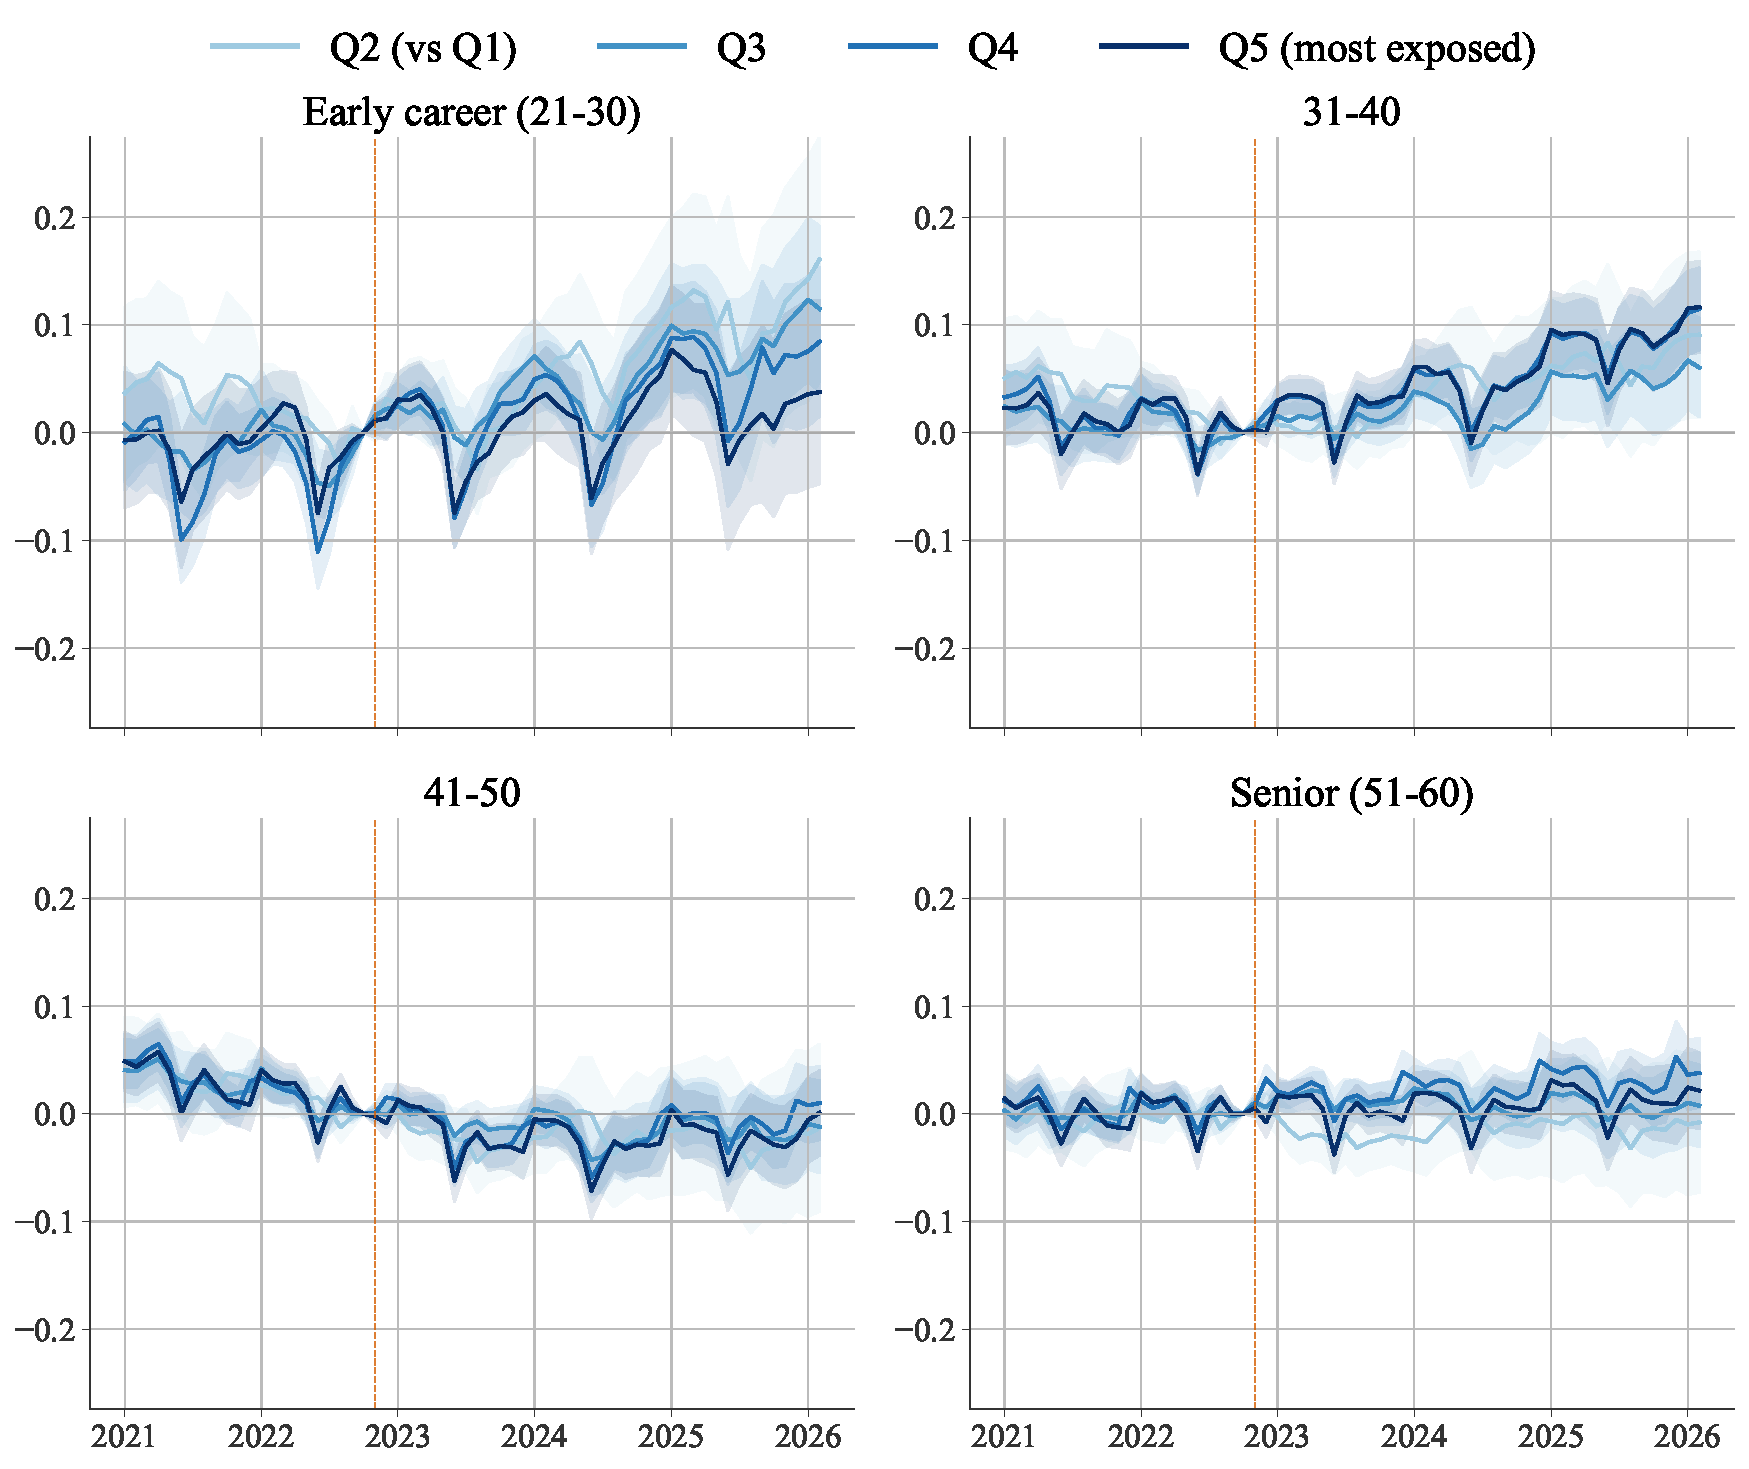
\includegraphics[height=5.5cm,keepaspectratio]{figure_firmfe_poisson_es_grid.pdf}

\vspace{0.2em}
\footnotesize
Q2--Q5 vs.\ Q1 by decade age group. At 21--30, Q5 is noisy and ends slightly positive; 31--40 rises to about $+0.12$; 41--50 drifts negative through 2025 and recovers to near zero; 51--60 stays flat. Collapsed Q5 $\times$ Post: $+0.013$ (n.s.), $+0.050$***, $-0.021$*, $+0.007$.
\end{frame}

% ---------------------------------------------------------------
\begin{frame}{Cell vs.\ within-firm: same story}
\centering
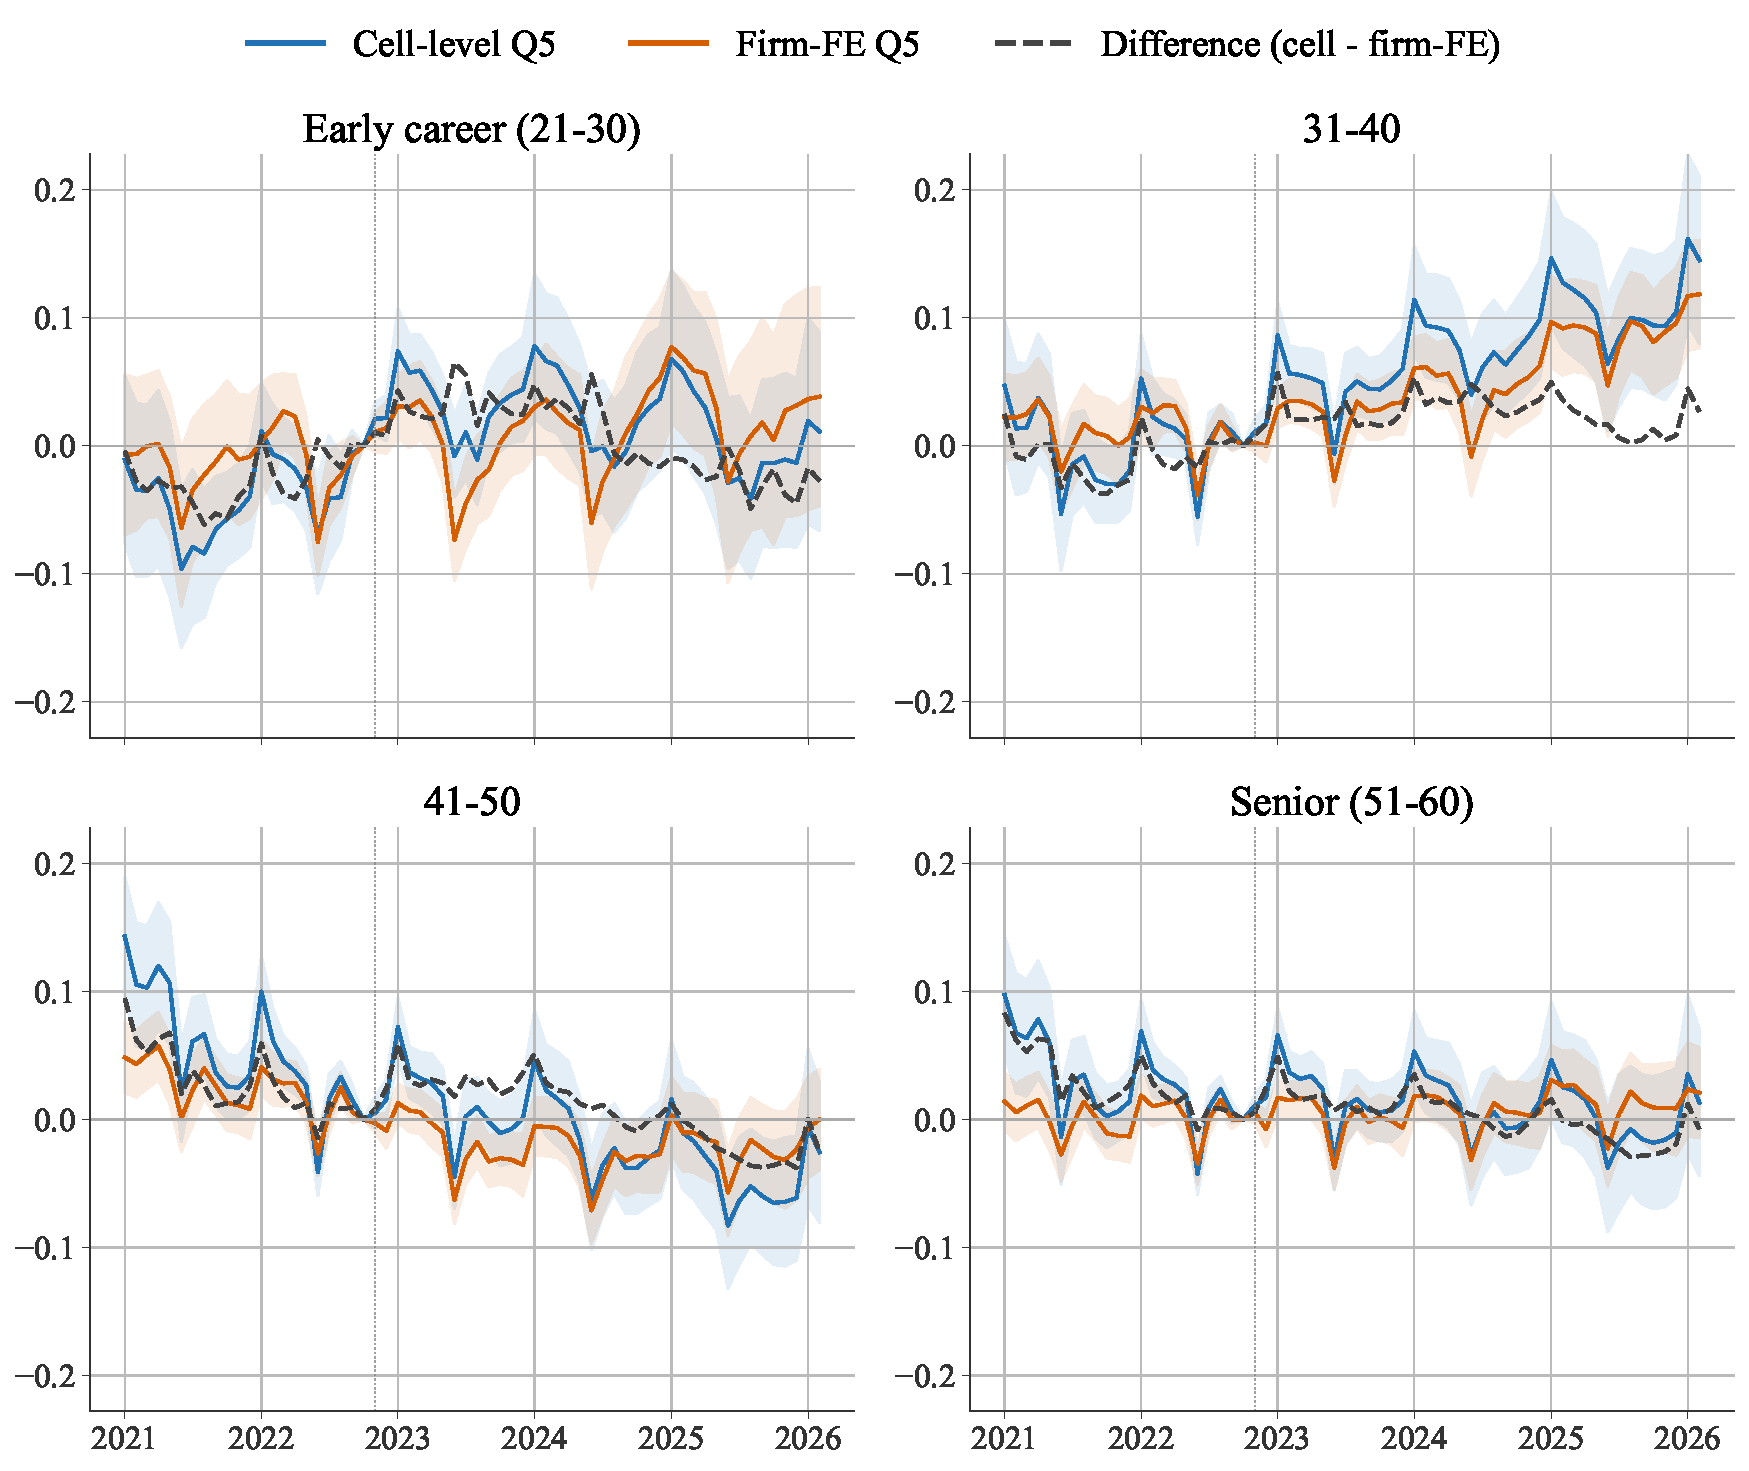
\includegraphics[height=5.5cm,keepaspectratio]{figure_cell_vs_firmfe_q5_grid.pdf}

\vspace{0.2em}
\footnotesize
Nested reconciliation of the Q5 estimates: switching data source moves nothing ($\leq 0.003$ in any age group); the $\geq 20$-worker restriction is small; the largest single step is cell to firm-FE, mainly at 31--40 ($+0.084 \to +0.050$). Signs unchanged throughout.
\end{frame}

% ---------------------------------------------------------------
\begin{frame}{Replicating Brynjolfsson et al.\ (ages 22--25)}
\centering
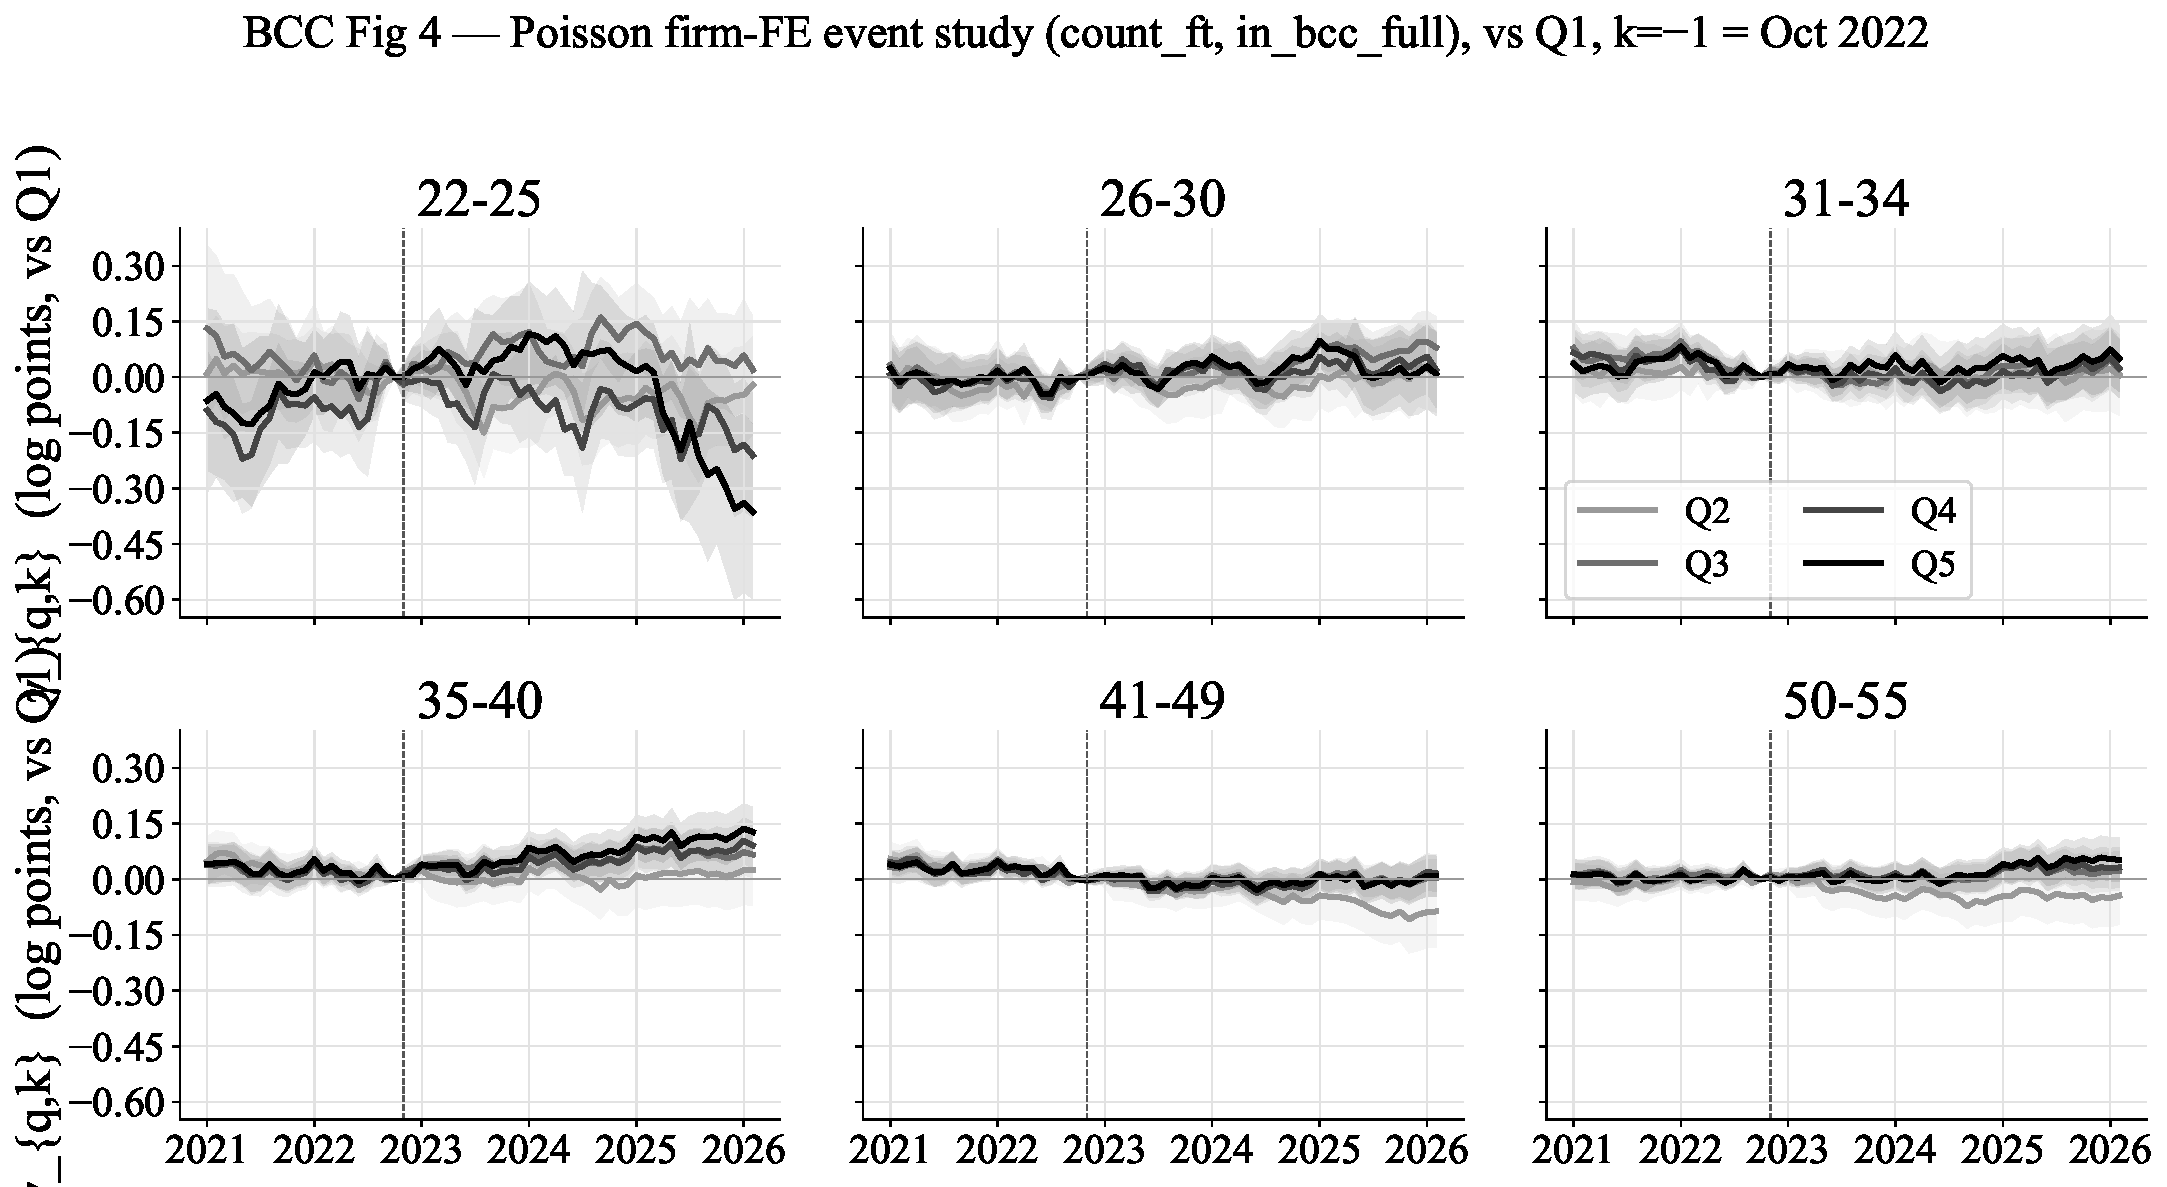
\includegraphics[height=5.1cm,keepaspectratio]{fig_bcc_4_es.pdf}

\vspace{0.2em}
\footnotesize
Balanced panel of full-time private-sector workers, six age bins. For ages 22--25 the average post-ChatGPT Q5 vs.\ Q1 gap is small ($\sim 3$ log points), but Q5 falls below Q1 from spring 2025, widening to about 35 log points by February 2026, more than the 15 reported for the US. Late, imprecise, and on rejected pre-trends.
\end{frame}


% ---------------------------------------------------------------
\section{Cross-country comparison}
% Discussion (frames removed: Alternative explanations, Cross-country).


% ---------------------------------------------------------------
\section{The dashboard: kiindeksen.no}
% The public dashboard: kiindeksen.no

\begin{frame}{Employment change by quintile since ChatGPT}
\centering
\begin{tabular}{lccccc}
\toprule
 & Q1 & Q2 & Q3 & Q4 & Q5 \\
\midrule
Average change (\%) & -0.63 & +2.94 & +0.95 & +2.86 & -0.09 \\
\addlinespace
Difference vs.\ Q1 (\%) & --- & +3.57 & +1.59 & +3.49 & +0.54 \\
 &  & (5.36) & (2.67) & (2.15) & (2.42) \\
\midrule
Occupations & \multicolumn{5}{c}{374} \\
\bottomrule
\end{tabular}


\vspace{0.8em}
\footnotesize
Change from October 2022 to the February--April 2026 average; seasonally adjusted private-sector headcount, ages 21--60, occupations weighted by October 2022 employment (Yagan 2019 style). Most exposed $-0.09\,\%$ vs.\ least exposed $-0.63\,\%$: a $+0.54$ pp double difference (SE 2.42), not significant. Robust SEs across occupations in parentheses.
\end{frame}

% ---------------------------------------------------------------
\begin{frame}{kiindeksen.no: a live index}
\centering
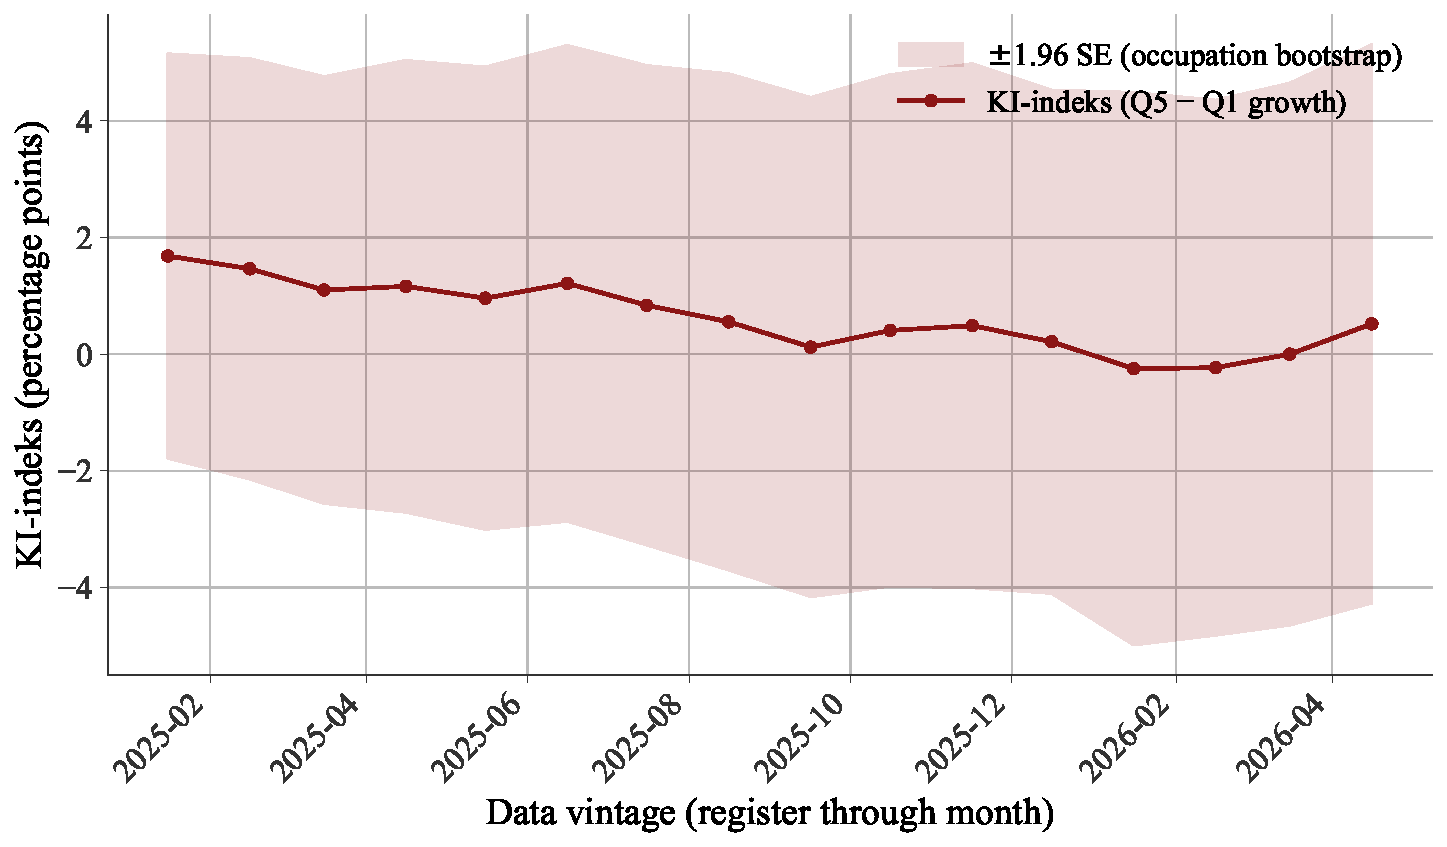
\includegraphics[height=5.2cm,keepaspectratio]{figure_recursive_kiindeks_ci.pdf}

\vspace{0.2em}
\footnotesize
The headline ``KI-indeks'': Q5 vs.\ Q1 employment growth, most recent three months vs.\ October 2022. Across expanding data vintages it drifts from $+1.7$ to $-0.2$ and back to $+0.5$ pp (April 2026). Bootstrap SE of 2 to 2.5 pp throughout: never statistically distinguishable from zero. A genuine change = a sustained move beyond the band.
\end{frame}


% ---------------------------------------------------------------
\section{Conclusion}
% Conclusion

\begin{frame}{Takeaway}
\small
\begin{itemize}\setlength{\itemsep}{5pt}
  \item \textbf{No aggregate job crisis.} Private-sector employment is growing; the employment rate is stable.
  \item \textbf{Full distribution.} Since October 2022, employment fell 0.1\,\% in the most exposed occupations against 0.6\,\% in the least exposed: a $+0.5$ pp gap, well within the $\sim$2.5 pp bootstrap SE.
  \item \textbf{The canary is real but does not generalize.} Young workers in software development and customer service fell after ChatGPT; across full exposure quintiles, Q5 did not fall behind Q1 at ages 21--30. Pre-trends warrant caution in both directions.
  \item \textbf{Cross-country.} Norway resembles the US and Sweden on case studies, Denmark and Finland on systematic evidence.
  \item \textbf{Monitoring continues} monthly at kiindeksen.no ($\sim$3-month data lag). All results private sector.
\end{itemize}
\end{frame}


% ---------------------------------------------------------------
\section*{Backup}
% Robustness

\begin{frame}{Population and cohort adjustment}
\centering
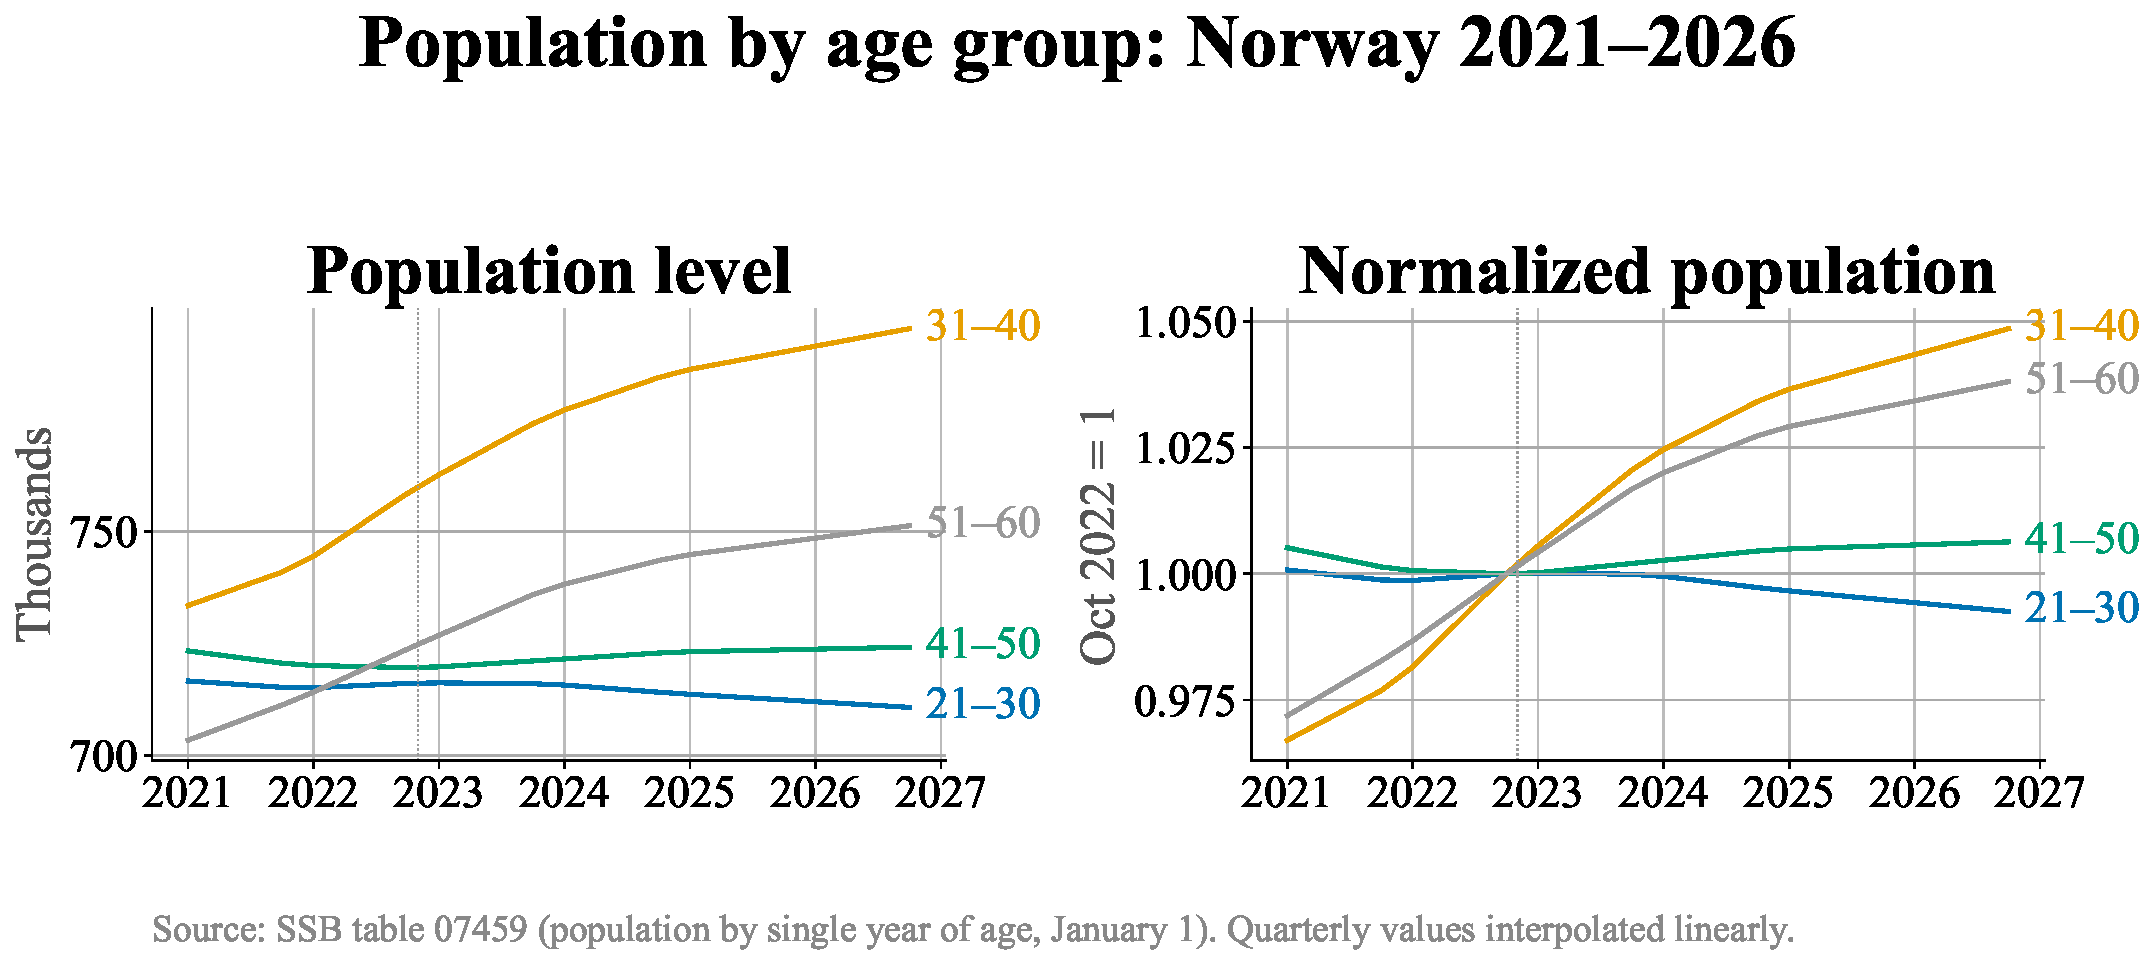
\includegraphics[height=5cm,keepaspectratio]{figureA0b_cohort_sizes.pdf}

\vspace{0.5em}
\begin{itemize}\setlength{\itemsep}{4pt}
  \item Per-capita normalisation (divide by SSB resident population in the same age cell).
  \item Composition adjustment fixes the within-bin age distribution at 2021-Q1.
  \item The age-by-quintile pattern is unchanged after both adjustments.
\end{itemize}
\end{frame}

% Backup slides: each carries a \hypertarget so it can be linked to from the
% main flow, and a \beamerbutton{Back} that returns to the slide it was
% reached from.

\begin{frame}{Lindenlaub et al.\ (2026), Fig.\ 1: AI adoption vs.\ four exposure measures}
\hypertarget{lorv-detail}{}
\centering
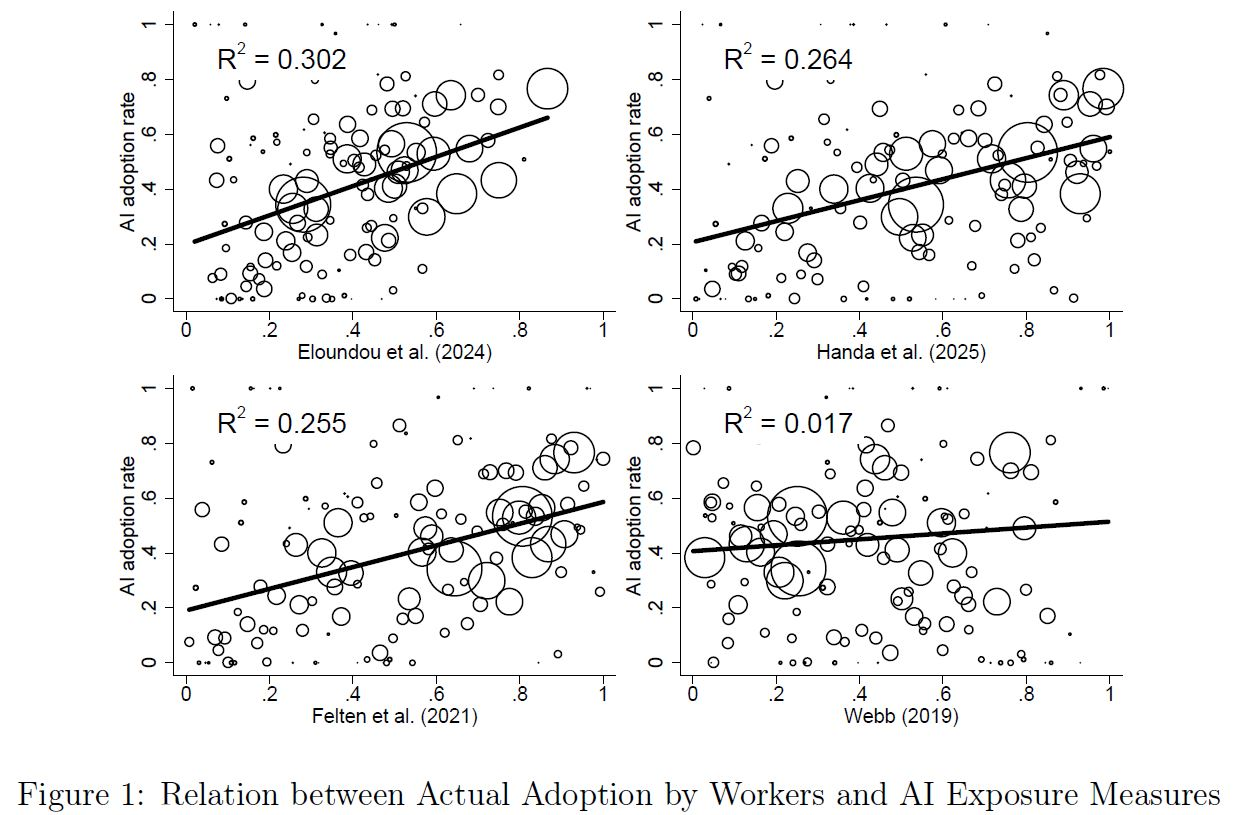
\includegraphics[height=5.4cm,keepaspectratio]{LORV_Fig1_Actual_adoptoin_vs_Exposure.JPG}

\vspace{0.3em}
\footnotesize
Each panel regresses worker-reported AI adoption on an exposure measure. Eloundou et al.\ has $R^2 = 0.30$, ahead of Handa (0.26), Felten (0.26), and Webb (0.02).

\vspace{0.3em}
\hfill\hyperlink{after-eloundou}{\beamerbutton{Back}}
\end{frame}

% ---------------------------------------------------------------
\begin{frame}{Public sector: no exposure gradient}
\hypertarget{public-sector-detail}{}
\centering
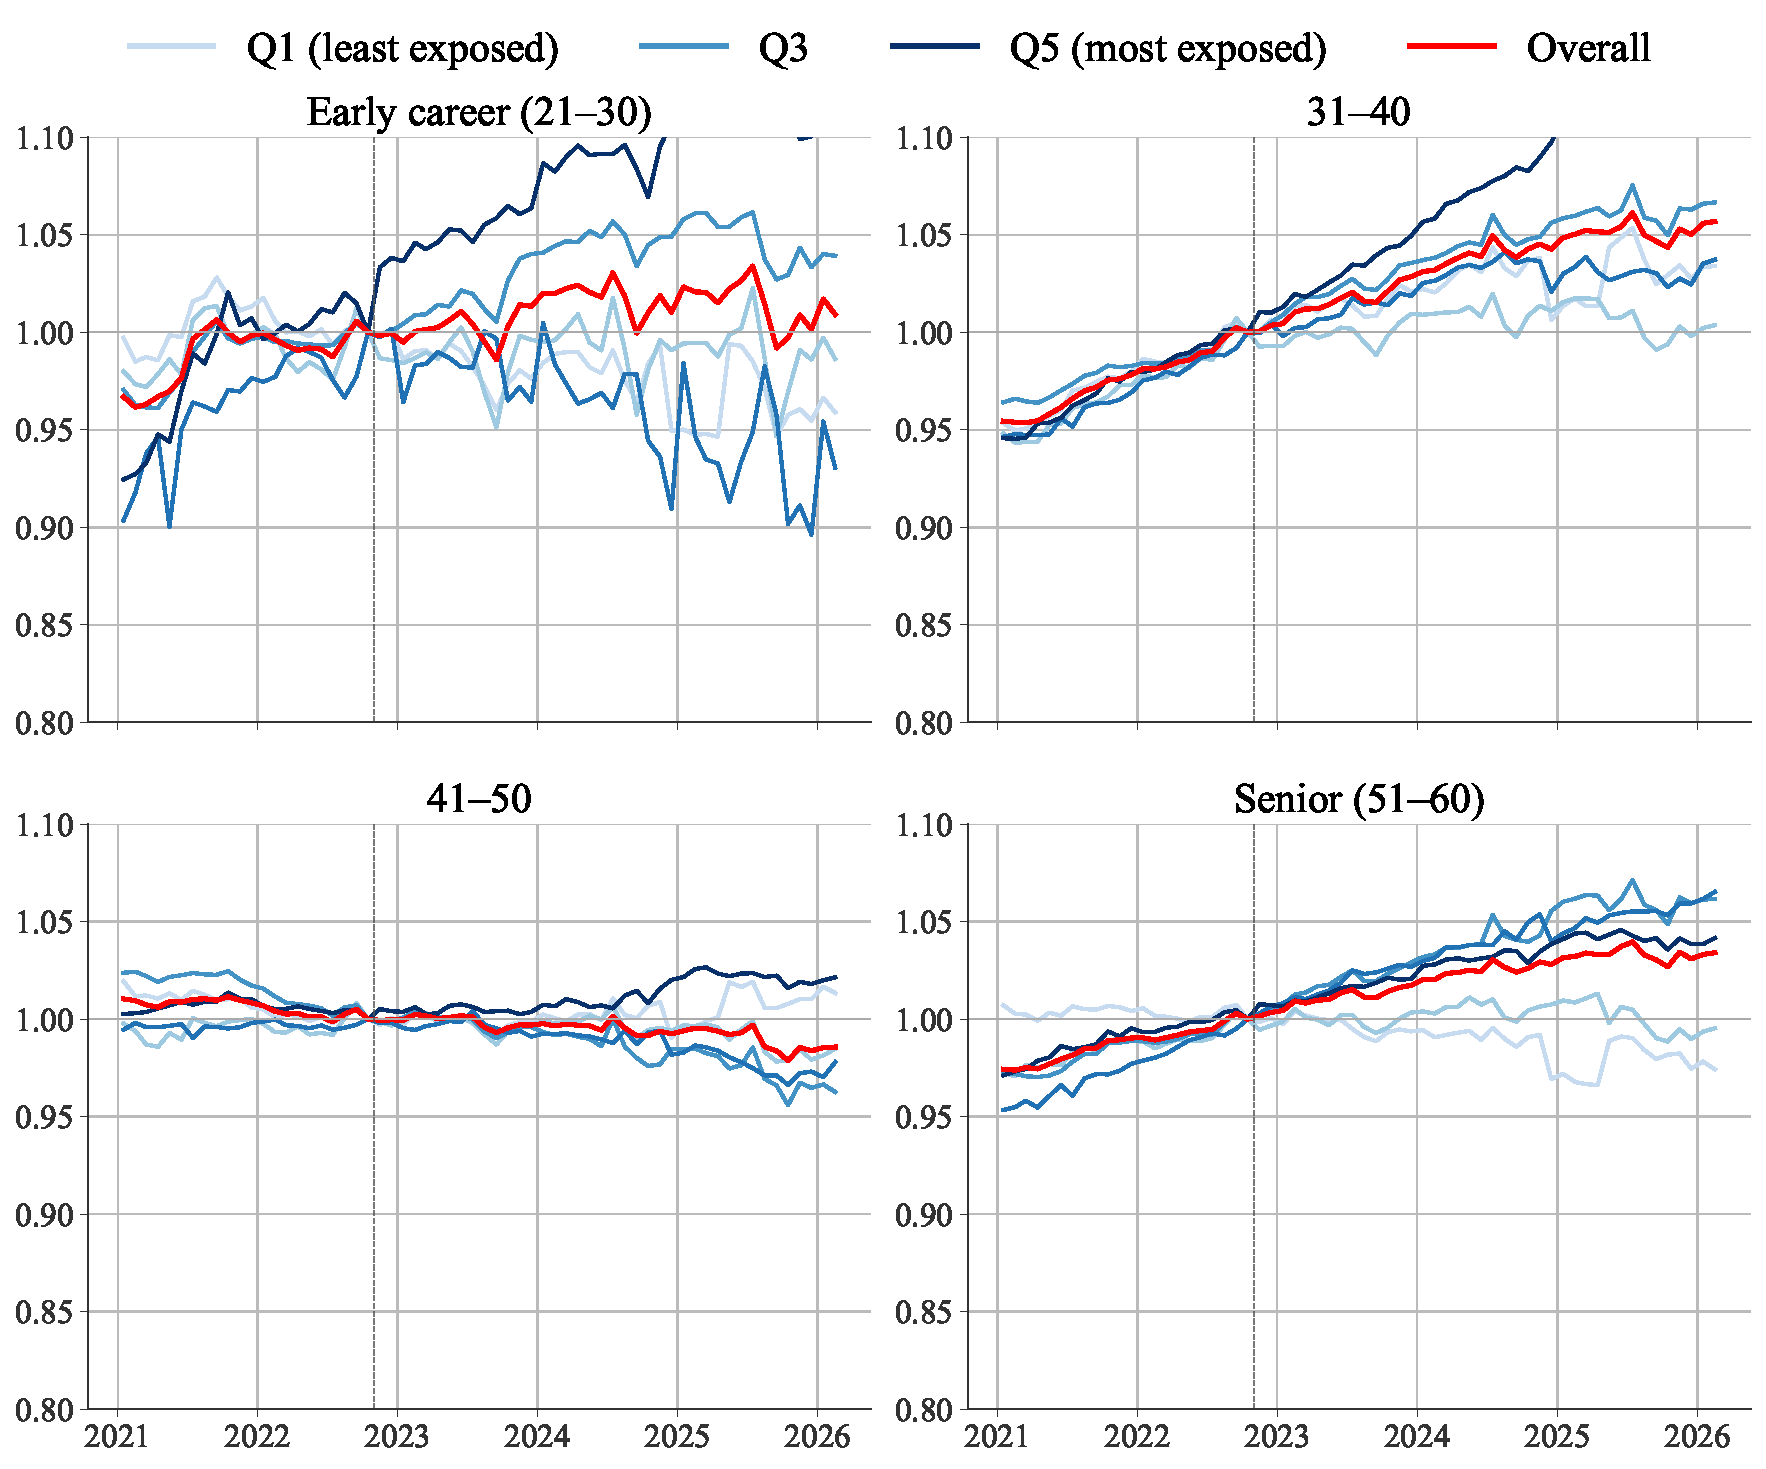
\includegraphics[height=5.5cm,keepaspectratio]{figure_emp_decade_public_sa.pdf}

\vspace{0.3em}
\footnotesize
Same indexed series as the private-sector slide, public sector, seasonally adjusted. No exposure gradient at any age.

\vspace{0.3em}
\hfill\hyperlink{after-private}{\beamerbutton{Back}}
\end{frame}

% ---------------------------------------------------------------
\begin{frame}{Cash earnings: no divergence}
\hypertarget{cash-earnings-detail}{}
\centering
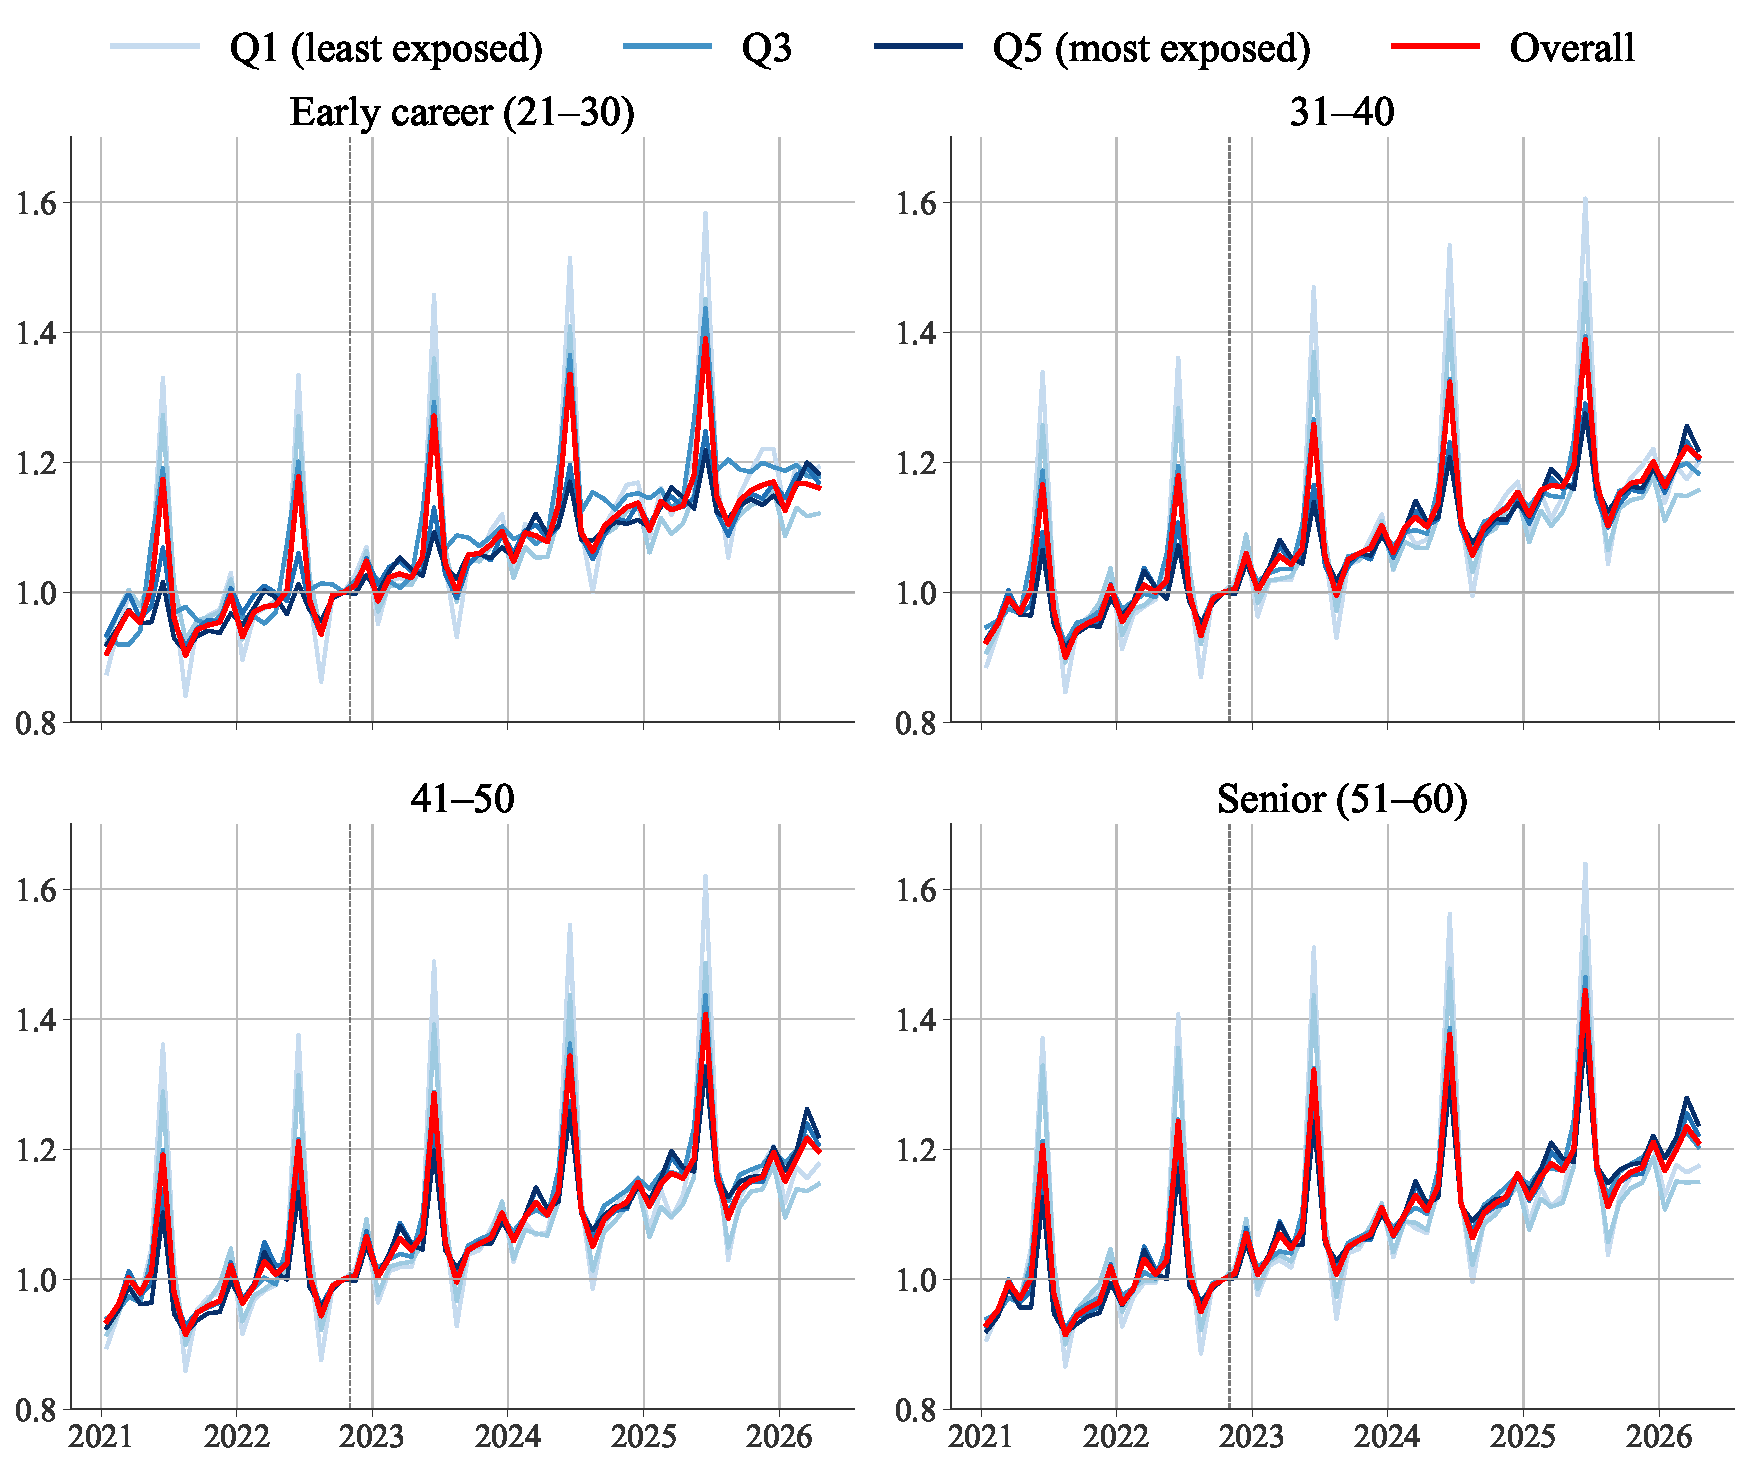
\includegraphics[height=5.2cm,keepaspectratio]{figure_kontantlonn_decade_private.pdf}

\vspace{0.2em}
\footnotesize
Cash earnings (\emph{kontantlønn}) by quintile and age, private sector. Seasonal patterns dominate (holiday pay, December bonuses): a tentative null, consistent with adjustment on the hiring margin under two-tier bargaining.

\vspace{0.3em}
\hfill\hyperlink{after-private}{\beamerbutton{Back}}
\end{frame}

% ---------------------------------------------------------------
\begin{frame}{Handa augmentation: no gradient}
\hypertarget{handa-aug-detail}{}
\centering
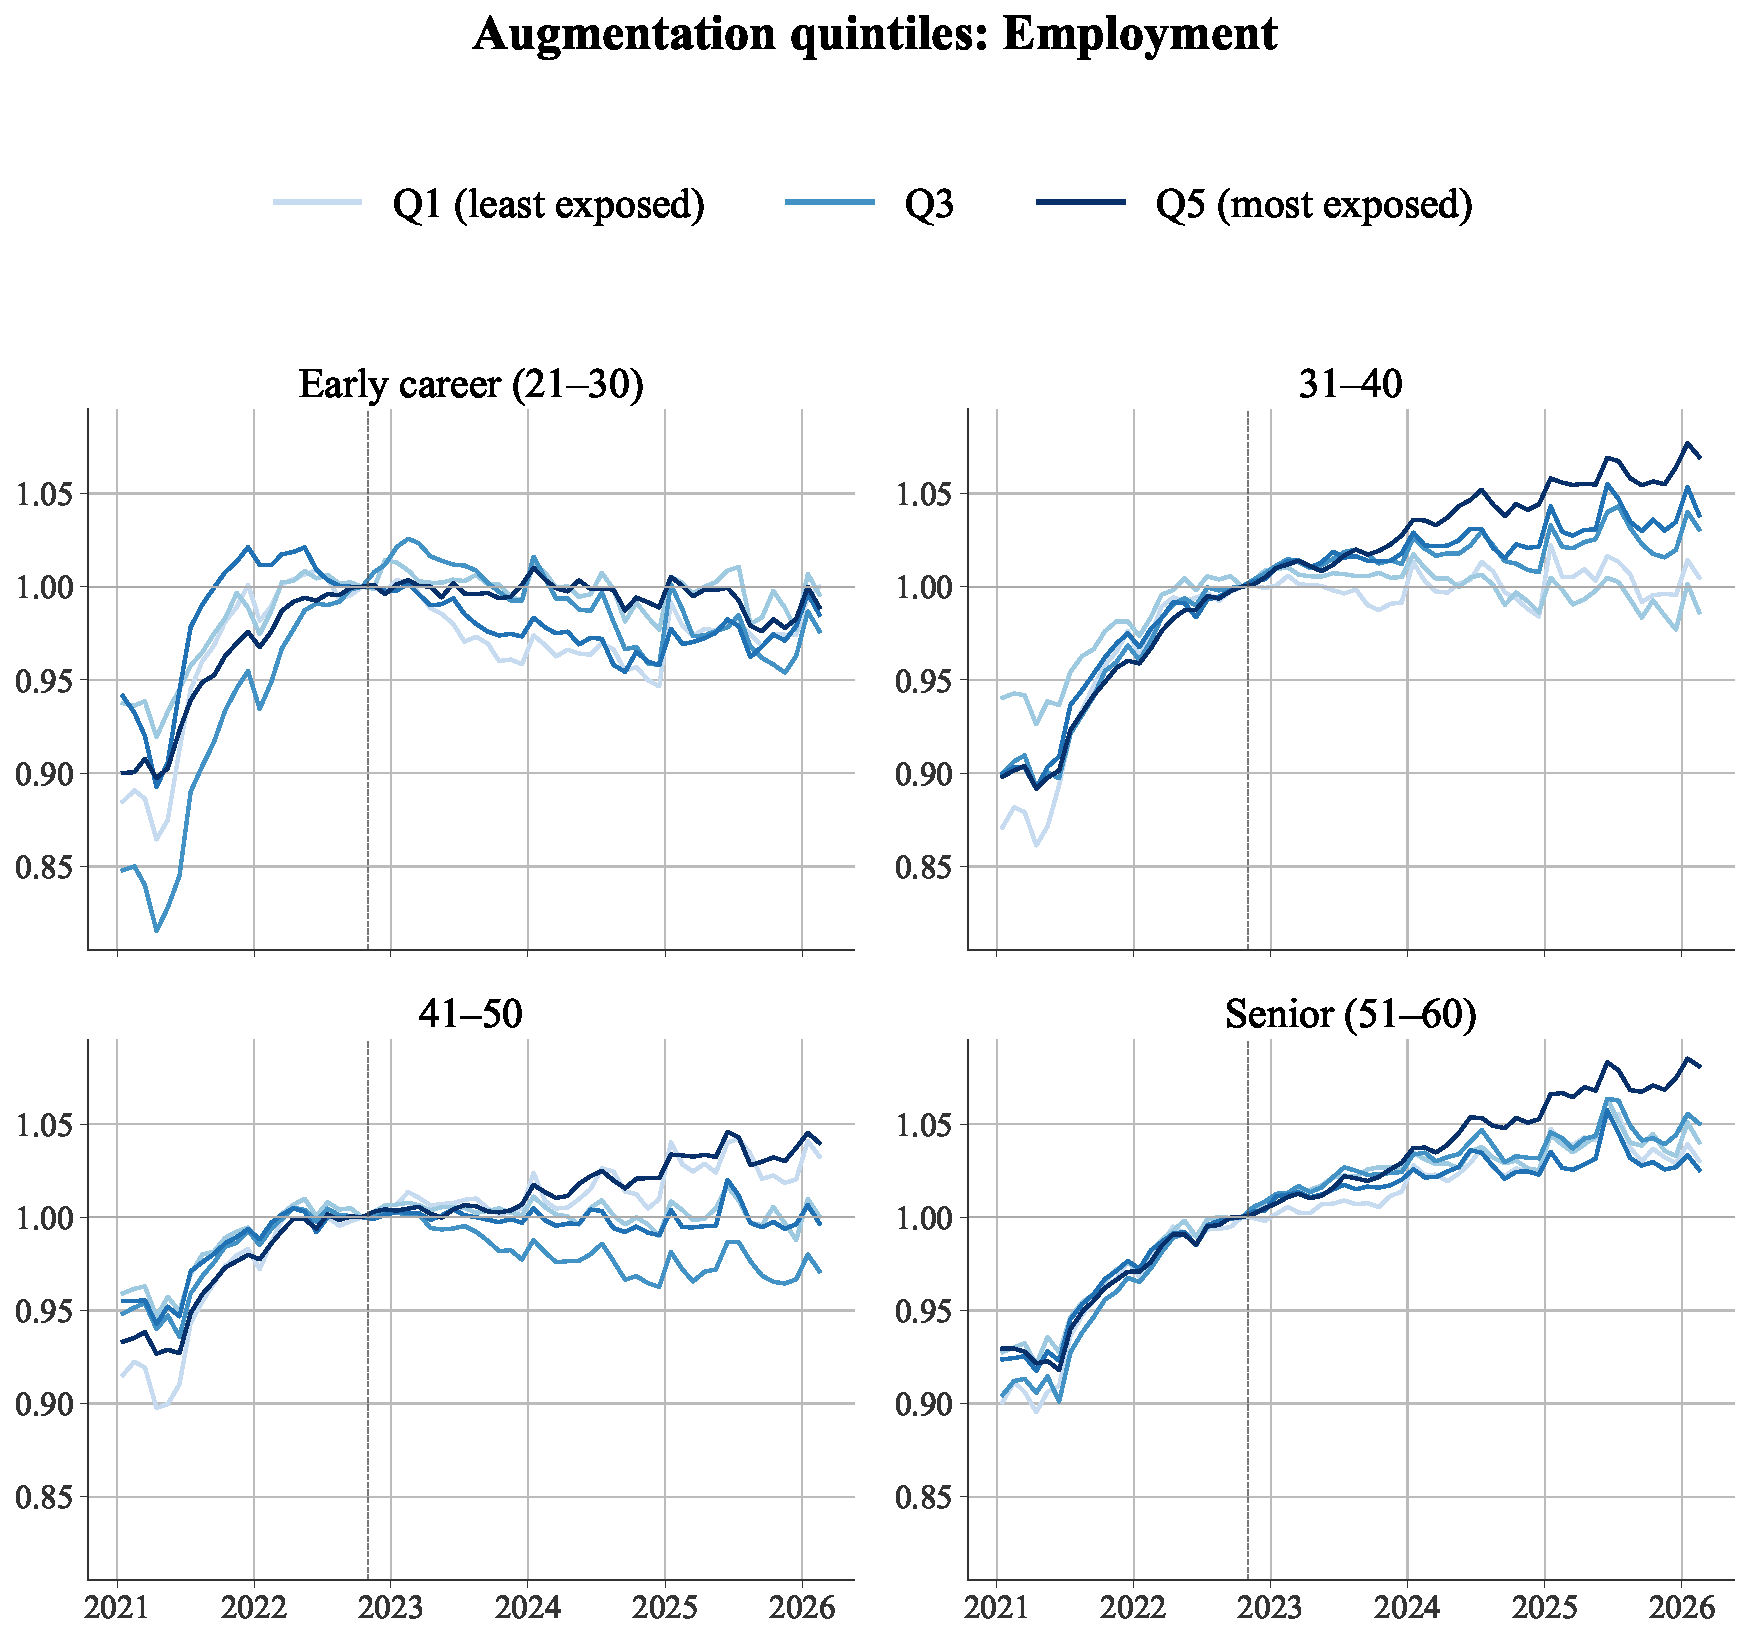
\includegraphics[height=5.5cm,keepaspectratio]{figure_age_by_quintile_handa_aug_sa.pdf}

\vspace{0.3em}
\footnotesize
Quintiles ranked by \textbf{augmentation} share of Claude usage, seasonally adjusted. Gaps are less pronounced than for automation; the least exposed are sometimes on par with the most exposed.

\vspace{0.3em}
\hfill\hyperlink{after-handa}{\beamerbutton{Back}}
\end{frame}

% ---------------------------------------------------------------
\begin{frame}{Cell-level event study, Q3 reference}
\hypertarget{cell-es-q3-detail}{}
\centering
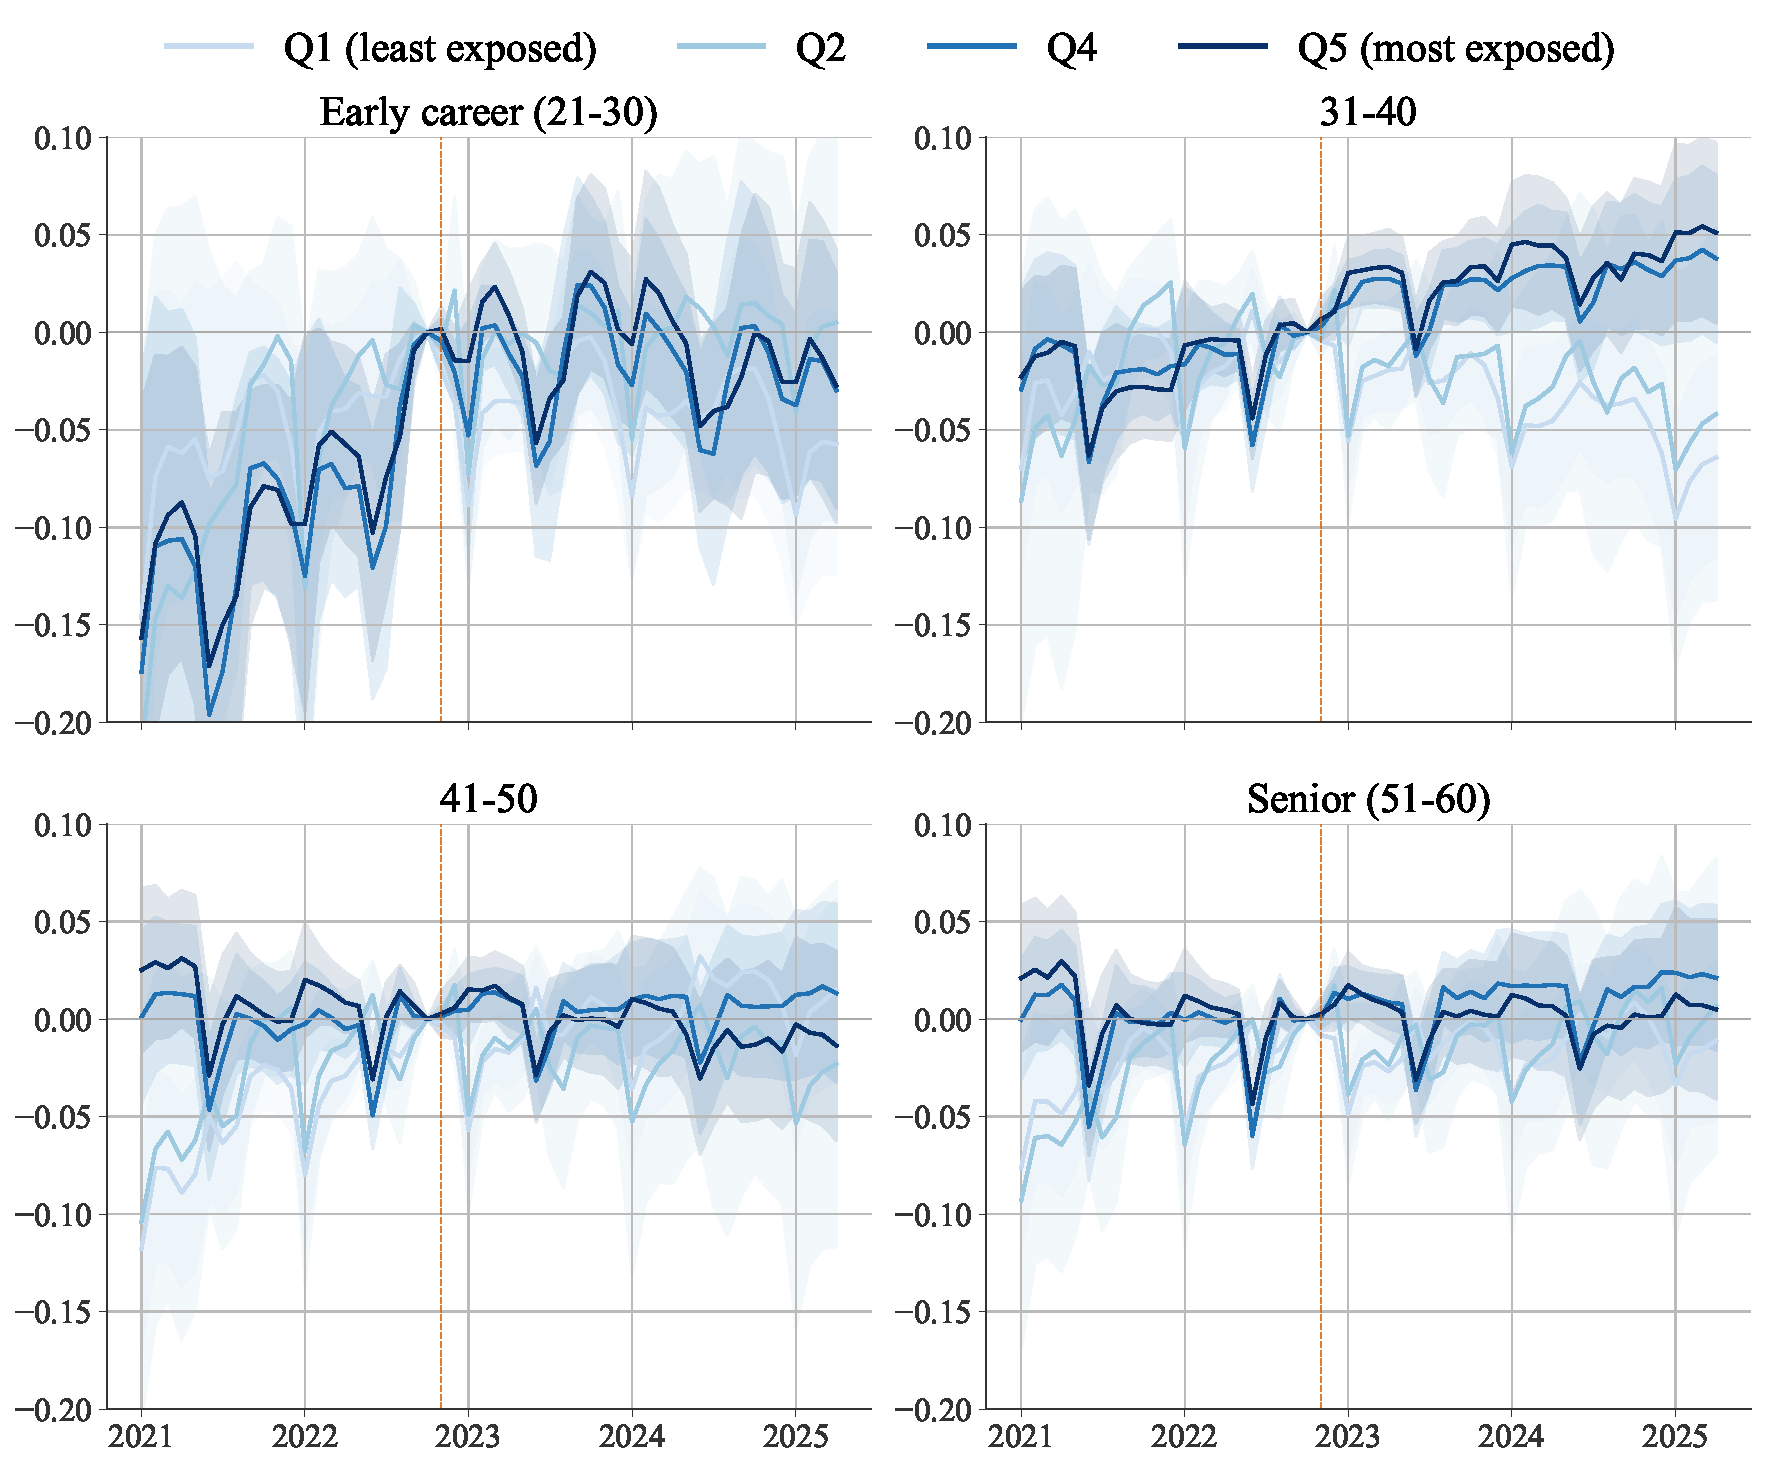
\includegraphics[height=5.5cm,keepaspectratio]{figure_microdata_poisson_es_grid_q3.pdf}

\vspace{0.3em}
\footnotesize
Same cell-level Poisson event study, plotted against Q3 (median exposure) instead of Q1. Q3 avoids Q1's winter-construction seasonality; the qualitative pattern is unchanged.

\vspace{0.3em}
\hfill\hyperlink{after-cell-did}{\beamerbutton{Back}}
\end{frame}

% ---------------------------------------------------------------
% Worked examples from the mapping deck.
\begin{frame}{Backup: mapping worked examples}
\hypertarget{worked-examples}{}
\begin{itemize}\setlength{\itemsep}{6pt}
  \item Five further one-to-one occupations, with full task tables: carpenters, secondary teachers, lawyers, economists, ICT operations technicians.
  \item A many-to-one example (STYRK 1112) and the O*NET data structure.
\end{itemize}

\vspace{0.3em}
\hfill\hyperlink{after-mapping}{\beamerbutton{Back}}
\end{frame}

% Eloundou et al. (2024): additional worked-example frames
% (split out of eloundou.tex; input by the mapping deck and presentation backup)

\begin{frame}{Other one-to-one mappings (large Norwegian occupations)}
\centering\footnotesize
\setlength{\tabcolsep}{4pt}
\begin{tabular}{llp{4.4cm}rcc}
\toprule
STYRK & Norwegian title & SOC 2010 (US title) & employed & $\beta_{\text{occ}}$ & Q \\
\midrule
7115 & Tømrere og snekkere               & 47-2031 Carpenters                  & 47{,}106 & 0.144 & 2 \\
2330 & Lektorer (videregående skole)     & 25-2031 Secondary teachers          & 31{,}155 & 0.333 & 3 \\
2611 & Jurister og advokater             & 23-1011 Lawyers                     & 11{,}808 & 0.425 & 4 \\
2631 & Forskere/rådgivere, samf.økonomi  & 19-3011 Economists                  &  1{,}282 & 0.553 & 5 \\
3511 & Driftsteknikere, IKT              & 43-9011 Computer Operators          & 16{,}517 & 0.736 & 5 \\
\bottomrule
\end{tabular}

\vspace{1em}
All five are clean one-to-one in the BLS crosswalk. Exposure spans Q2 to Q5: carpenters at the bottom, ICT operations technicians at the top. $\beta_{\text{occ}}$ is taken from the published Core-weighted occupation file, so it can differ slightly from an unweighted task mean. SOC titles do not always match the Norwegian title literally (e.g.\ ``Computer Operators'' vs.\ ``Driftsteknikere, IKT'').
\end{frame}

% Worked examples for the five additional one-to-one occupations from the
% "Other one-to-one mappings" slide. Each occupation gets a chain slide and a
% full task-list slide, except STYRK 3511 (Driftsteknikere, IKT), where the
% SOC 2010 → 2018 re-coding fans out to nine O*NET specialties.

% =================================================================
% STYRK 7115: Tømrere og snekkere (Carpenters)
% =================================================================
\begin{frame}{Worked example: Tømrere og snekkere (STYRK 7115)}
\centering
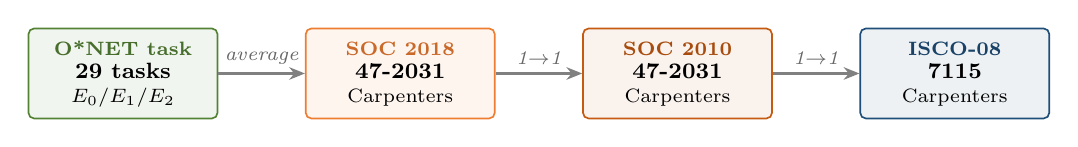
\begin{tikzpicture}[node distance=1.0cm and 1.1cm]
  \node[codebox=cTASK] (task) {\cbox{cTASK}{O*NET task}{29 tasks}{$E_0/E_1/E_2$}};
  \node[codebox=cSOC18, right=of task] (soc18) {\cbox{cSOC18}{SOC 2018}{47-2031}{Carpenters}};
  \node[codebox=cSOC10, right=of soc18] (soc10) {\cbox{cSOC10}{SOC 2010}{47-2031}{Carpenters}};
  \node[codebox=cSTYRK, right=of soc10] (isco) {\cbox{cSTYRK}{ISCO-08}{7115}{Carpenters}};

  \draw[chain] (task) -- node[arrowlabel]{average} (soc18);
  \draw[chain] (soc18) -- node[arrowlabel]{1$\to$1} (soc10);
  \draw[chain] (soc10) -- node[arrowlabel]{1$\to$1} (isco);
\end{tikzpicture}

\vspace{0.8em}
STYRK 7115 is Tømrere og snekkere. Same 6-digit SOC in both vintages, one O*NET specialty, 29 tasks. Mostly $E_0$: physical work dominates.
\end{frame}

% task table
\begin{frame}{Task-level scoring: Carpenters (SOC 47-2031, 29 tasks)}
\centering\tiny
\setlength{\tabcolsep}{4pt}
\renewcommand{\arraystretch}{1.05}
\begin{tabular}{p{5.4cm}cc @{\hspace{0.3cm}} p{5.4cm}cc}
\toprule
O*NET task & $E$ & $\beta$ & O*NET task & $E$ & $\beta$ \\
\midrule
Follow safety rules and regulations           & $E_0$ & 0.0 & Dig or direct digging of post holes        & $E_0$ & 0.0 \\
Measure and mark cutting lines on materials   & $E_0$ & 0.0 & Cover subfloors with building paper        & $E_0$ & 0.0 \\
Assemble and fasten materials                 & $E_0$ & 0.0 & Construct forms or chutes for concrete     & $E_0$ & 0.0 \\
\rO{Study specifications in blueprints}{$E_2$}{0.5}            & \rO{Arrange for subcontractors}{$E_2$}{0.5} \\
Shape or cut materials to measurements        & $E_0$ & 0.0 & Build or repair cabinets, doors, floors    & $E_0$ & 0.0 \\
Verify trueness with plumb bob and level      & $E_0$ & 0.0 & Finish surfaces of woodwork or wallboard   & $E_0$ & 0.0 \\
\rO{Inspect ceiling/floor tile, wall coverings}{$E_2$}{0.5}    & \rO{Select and order lumber and materials}{$E_2$}{0.5} \\
Erect scaffolding or ladders                  & $E_0$ & 0.0 & Work with or remove hazardous material     & $E_0$ & 0.0 \\
Install windows, frames, fixtures             & $E_0$ & 0.0 & Fill cracks or defects in plaster          & $E_0$ & 0.0 \\
\rR{Maintain records, present written reports}{$E_1$}{1.0}     & \rO{Prepare cost estimates for clients}{$E_2$}{0.5} \\
Remove damaged or defective parts             & $E_0$ & 0.0 & Perform minor plumbing or concrete work    & $E_0$ & 0.0 \\
\rO{Maintain job records, schedule work crew}{$E_2$}{0.5}      & Apply shock-absorbing or sound-deadening   & $E_0$ & 0.0 \\
Anchor and brace forms and structures         & $E_0$ & 0.0 & Examine structural timbers for decay       & $E_0$ & 0.0 \\
Bore boltholes in timber/masonry/concrete     & $E_0$ & 0.0 & Build sleds from logs and timbers          & $E_0$ & 0.0 \\
Install rough door/window frames, subflooring & $E_0$ & 0.0 &                                            &       &      \\
\midrule
\multicolumn{6}{l}{\textbf{Counts:} 22 $E_0$ \quad 1 $E_1$ \quad 6 $E_2$ \qquad
                   \textbf{SOC $\beta$ (mean of 29 tasks): \;0.138 (Q2)}} \\
\bottomrule
\end{tabular}
\end{frame}


% =================================================================
% STYRK 2330: Lektorer videregående (Secondary teachers)
% =================================================================
\begin{frame}{Worked example: Lektorer videregående (STYRK 2330)}
\centering
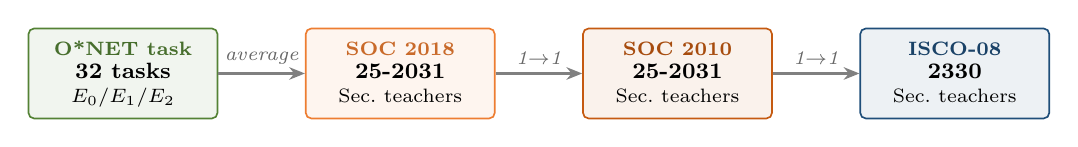
\begin{tikzpicture}[node distance=1.0cm and 1.1cm]
  \node[codebox=cTASK] (task) {\cbox{cTASK}{O*NET task}{32 tasks}{$E_0/E_1/E_2$}};
  \node[codebox=cSOC18, right=of task] (soc18) {\cbox{cSOC18}{SOC 2018}{25-2031}{Sec.\ teachers}};
  \node[codebox=cSOC10, right=of soc18] (soc10) {\cbox{cSOC10}{SOC 2010}{25-2031}{Sec.\ teachers}};
  \node[codebox=cSTYRK, right=of soc10] (isco) {\cbox{cSTYRK}{ISCO-08}{2330}{Sec.\ teachers}};

  \draw[chain] (task) -- node[arrowlabel]{average} (soc18);
  \draw[chain] (soc18) -- node[arrowlabel]{1$\to$1} (soc10);
  \draw[chain] (soc10) -- node[arrowlabel]{1$\to$1} (isco);
\end{tikzpicture}

\vspace{0.8em}
STYRK 2330 is Lektorer mv.\ (videregående skole). One O*NET specialty, 32 tasks. Most are $E_2$ (LLM with software is enough) and reflect classroom and administrative work.
\end{frame}

% task table
\begin{frame}{Task-level scoring: Secondary teachers (SOC 25-2031, 32 tasks)}
\centering\tiny
\setlength{\tabcolsep}{4pt}
\renewcommand{\arraystretch}{1.0}
\begin{tabular}{p{5.4cm}cc @{\hspace{0.3cm}} p{5.4cm}cc}
\toprule
O*NET task & $E$ & $\beta$ & O*NET task & $E$ & $\beta$ \\
\midrule
\rO{Instruct through lectures, discussions}{$E_2$}{0.5}          & Plan and conduct field trips                & $E_0$ & 0.0 \\
Establish rules of student behavior             & $E_0$ & 0.0 & Sponsor extracurricular activities          & $E_0$ & 0.0 \\
\rO{Prepare materials and classrooms}{$E_2$}{0.5}                & \rO{Perform administrative duties}{$E_2$}{0.5} \\
\rO{Adapt teaching to varying abilities}{$E_2$}{0.5}             & \rO{Prepare and implement remedial programs}{$E_2$}{0.5} \\
\rO{Observe and evaluate students' performance}{$E_2$}{0.5}      & Attend professional meetings and workshops  & $E_0$ & 0.0 \\
\rO{Establish clear objectives for lessons}{$E_2$}{0.5}          & \rO{Use computers and audiovisual aids}{$E_2$}{0.5} \\
\rO{Prepare students for later grades}{$E_2$}{0.5}               & \rO{Select, store, order, or use class materials}{$E_2$}{0.5} \\
\rO{Prepare, administer, and grade tests}{$E_2$}{0.5}            & \rO{Collaborate with other teachers}{$E_2$}{0.5} \\
\rO{Maintain accurate, complete records}{$E_2$}{0.5}             & \rO{Plan and supervise projects, field studies}{$E_2$}{0.5} \\
Enforce attendance and progression rules        & $E_0$ & 0.0 & Meet with professionals on programs         & $E_0$ & 0.0 \\
Instruct and monitor use of equipment           & $E_0$ & 0.0 & \rO{Guide and counsel students}{$E_2$}{0.5} \\
\rO{Prepare content for diverse-needs students}{$E_2$}{0.5}      & Confer with parents on progress             & $E_0$ & 0.0 \\
\rO{Assign and grade class work and homework}{$E_2$}{0.5}        & \rO{Meet with administrators on instruction}{$E_2$}{0.5} \\
\rO{Prepare reports on student progress}{$E_2$}{0.5}             & \rO{Prepare for assigned classes}{$E_2$}{0.5} \\
\rR{Keep informed about developments in education}{$E_1$}{1.0}   & \rO{Provide disabled students with devices}{$E_2$}{0.5} \\
\rO{Prepare objectives and outlines}{$E_2$}{0.5}                 & Administer standardized tests               & $E_0$ & 0.0 \\
\midrule
\multicolumn{6}{l}{\textbf{Counts:} 12 $E_0$ \quad 1 $E_1$ \quad 19 $E_2$ \qquad
                   \textbf{SOC $\beta$ (mean of 32 tasks): \;0.328 (Q3)}} \\
\bottomrule
\end{tabular}
\end{frame}


% =================================================================
% STYRK 2611: Jurister og advokater (Lawyers)
% =================================================================
\begin{frame}{Worked example: Jurister og advokater (STYRK 2611)}
\centering
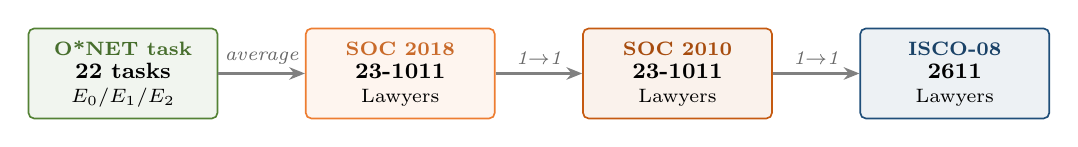
\begin{tikzpicture}[node distance=1.0cm and 1.1cm]
  \node[codebox=cTASK] (task) {\cbox{cTASK}{O*NET task}{22 tasks}{$E_0/E_1/E_2$}};
  \node[codebox=cSOC18, right=of task] (soc18) {\cbox{cSOC18}{SOC 2018}{23-1011}{Lawyers}};
  \node[codebox=cSOC10, right=of soc18] (soc10) {\cbox{cSOC10}{SOC 2010}{23-1011}{Lawyers}};
  \node[codebox=cSTYRK, right=of soc10] (isco) {\cbox{cSTYRK}{ISCO-08}{2611}{Lawyers}};

  \draw[chain] (task) -- node[arrowlabel]{average} (soc18);
  \draw[chain] (soc18) -- node[arrowlabel]{1$\to$1} (soc10);
  \draw[chain] (soc10) -- node[arrowlabel]{1$\to$1} (isco);
\end{tikzpicture}

\vspace{0.8em}
STYRK 2611 is Jurister og advokater. One O*NET specialty, 22 tasks. Nearly all tasks are $E_2$: text-heavy work where LLM plus software can substitute.
\end{frame}

% task table
\begin{frame}{Task-level scoring: Lawyers (SOC 23-1011, 22 tasks)}
\centering\tiny
\setlength{\tabcolsep}{4pt}
\renewcommand{\arraystretch}{1.15}
\begin{tabular}{p{5.4cm}cc @{\hspace{0.3cm}} p{5.4cm}cc}
\toprule
O*NET task & $E$ & $\beta$ & O*NET task & $E$ & $\beta$ \\
\midrule
\rO{Advise clients on legal rights}{$E_2$}{0.5}              & Confer with colleagues with specialties   & $E_0$ & 0.0 \\
Represent clients in court or in hearings   & $E_0$ & 0.0 & \rO{Examine legal data for advisability}{$E_2$}{0.5} \\
Select jurors, argue motions, meet judges   & $E_0$ & 0.0 & \rO{Search and examine public records}{$E_2$}{0.5} \\
\rO{Study Constitution, statutes, decisions}{$E_2$}{0.5}     & \rO{Act as trustee, guardian, or executor}{$E_2$}{0.5} \\
\rO{Prepare legal briefs and opinions}{$E_2$}{0.5}           & \rO{Help establish company legal policies}{$E_2$}{0.5} \\
\rO{Interpret laws, rulings, regulations}{$E_2$}{0.5}        & \rO{Negotiate settlements of civil disputes}{$E_2$}{0.5} \\
\rO{Prepare and draft legal documents}{$E_2$}{0.5}           & \rO{Probate wills, represent estate executors}{$E_2$}{0.5} \\
\rO{Present and summarize cases to judges}{$E_2$}{0.5}       & \rO{Work in environmental, public health law}{$E_2$}{0.5} \\
\rO{Gather evidence by interviewing clients}{$E_2$}{0.5}     & \rO{Perform administrative and management}{$E_2$}{0.5} \\
\rO{Analyze the probable outcomes of cases}{$E_2$}{0.5}      & \rO{Supervise legal assistants}{$E_2$}{0.5} \\
\rO{Evaluate findings; develop defense strategy}{$E_2$}{0.5} & \rO{Provide pro bono services}{$E_2$}{0.5} \\
\midrule
\multicolumn{6}{l}{\textbf{Counts:} 3 $E_0$ \quad 0 $E_1$ \quad 19 $E_2$ \qquad
                   \textbf{SOC $\beta$ (mean of 22 tasks): \;0.432 (Q4)}} \\
\bottomrule
\end{tabular}
\end{frame}


% =================================================================
% STYRK 2631: Forskere/rådgivere, samf.økonomi (Economists)
% =================================================================
\begin{frame}{Worked example: Forskere/rådgivere, samf.økonomi (STYRK 2631)}
\centering
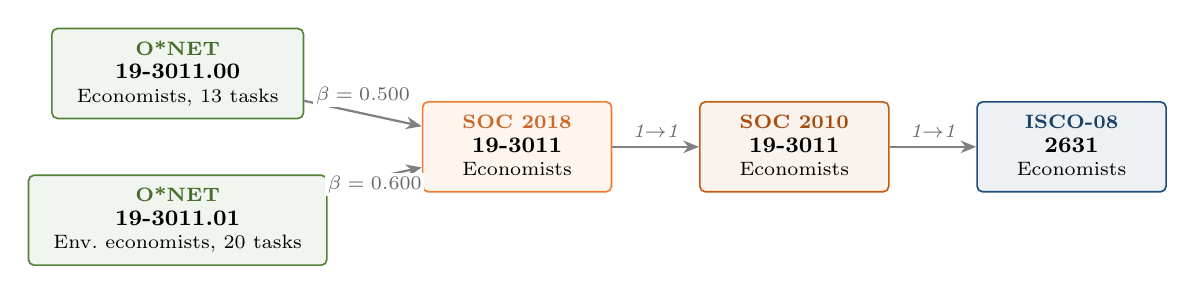
\begin{tikzpicture}[node distance=0.7cm and 1.1cm]
  \node[codebox=cTASK] (t1) {\cbox{cTASK}{O*NET}{19-3011.00}{Economists, 13 tasks}};
  \node[codebox=cTASK, below=of t1] (t2) {\cbox{cTASK}{O*NET}{19-3011.01}{Env.\ economists, 20 tasks}};

  \node[codebox=cSOC18, right=3.1cm of $(t1)!0.5!(t2)$] (soc18) {\cbox{cSOC18}{SOC 2018}{19-3011}{Economists}};
  \node[codebox=cSOC10, right=of soc18] (soc10) {\cbox{cSOC10}{SOC 2010}{19-3011}{Economists}};
  \node[codebox=cSTYRK, right=of soc10] (isco) {\cbox{cSTYRK}{ISCO-08}{2631}{Economists}};

  \draw[chain] (t1) -- node[arrowlabel,above]{$\beta = 0.500$} (soc18);
  \draw[chain] (t2) -- node[arrowlabel,below]{$\beta = 0.600$} (soc18);
  \draw[chain] (soc18) -- node[arrowlabel]{1$\to$1} (soc10);
  \draw[chain] (soc10) -- node[arrowlabel]{1$\to$1} (isco);
\end{tikzpicture}

\vspace{0.5em}
Two O*NET specialties roll up to one SOC 2018 code. The SOC-level $\beta$ averages the two specialty means: $(0.500 + 0.600)/2 = 0.550$, regardless of how many tasks each specialty contains.
\end{frame}

% task table
\begin{frame}{Task-level scoring: Economists (SOC 19-3011, 33 tasks across 2 specialties)}
\centering\tiny
\setlength{\tabcolsep}{4pt}
\renewcommand{\arraystretch}{1.0}
\begin{tabular}{p{5.4cm}cc @{\hspace{0.3cm}} p{5.4cm}cc}
\toprule
\multicolumn{3}{l}{\textbf{19-3011.00 Economists (13 tasks)}} & \multicolumn{3}{l}{\textbf{19-3011.01 Env.\ Economists (20 tasks)}} \\
\midrule
\rO{Study economic and statistical data}{$E_2$}{0.5}           & \rO{Prepare and deliver presentations}{$E_2$}{0.5} \\
\rO{Conduct research on economic issues}{$E_2$}{0.5}           & \rO{Develop programs or policy recommendations}{$E_2$}{0.5} \\
\rO{Compile, analyze, report data}{$E_2$}{0.5}                 & \rO{Develop economic models and forecasts}{$E_2$}{0.5} \\
\rO{Supervise research projects}{$E_2$}{0.5}                   & \rO{Demonstrate economic benefits of policies}{$E_2$}{0.5} \\
\rO{Teach theories and methods of economics}{$E_2$}{0.5}       & \rO{Conduct research on environmental relations}{$E_2$}{0.5} \\
\rO{Study impacts of public policies}{$E_2$}{0.5}              & \rR{Perform complex mathematical analyses}{$E_1$}{1.0} \\
\rO{Formulate recommendations and plans}{$E_2$}{0.5}           & \rR{Write social, legal, economic impact reports}{$E_1$}{1.0} \\
\rO{Explain economic impact of policies}{$E_2$}{0.5}           & \rO{Teach courses in environmental economics}{$E_2$}{0.5} \\
\rO{Provide advice and consultation}{$E_2$}{0.5}               & \rO{Develop programs to promote sustainability}{$E_2$}{0.5} \\
\rO{Forecast production and consumption}{$E_2$}{0.5}           & \rO{Develop systems for analyzing data}{$E_2$}{0.5} \\
\rO{Develop economic guidelines and standards}{$E_2$}{0.5}     & \rR{Write research proposals and grants}{$E_1$}{1.0} \\
\rO{Testify at regulatory or legislative hearings}{$E_2$}{0.5} & \rO{Examine exhaustibility of natural resources}{$E_2$}{0.5} \\
\rO{Provide litigation support}{$E_2$}{0.5}                    & \rO{Monitor or analyze market and env.\ trends}{$E_2$}{0.5} \\
\rR{Write technical documents or articles}{$E_1$}{1.0}         & \rO{Develop environmental research project plans}{$E_2$}{0.5} \\
                                              &       &     & \rO{Conduct research on economic, env.\ topics}{$E_2$}{0.5} \\
                                              &       &     & \rO{Collect and analyze data on env.\ impact}{$E_2$}{0.5} \\
                                              &       &     & \rO{Assess costs and benefits of activities}{$E_2$}{0.5} \\
                                              &       &     & \rO{Identify environmentally friendly business}{$E_2$}{0.5} \\
                                              &       &     & \rO{Interpret indicators of ecosystem health}{$E_2$}{0.5} \\
                                              &       &     & \rO{Collaborate with researchers across fields}{$E_2$}{0.5} \\
\midrule
\multicolumn{3}{l}{\textbf{Specialty mean:} \;0.500} & \multicolumn{3}{l}{\textbf{Specialty mean:} \;0.600} \\
\multicolumn{6}{l}{\textbf{SOC $\beta$} $= (0.500 + 0.600)/2 = $ \textbf{0.550 (Q5)}} \\
\bottomrule
\end{tabular}
\end{frame}


% =================================================================
% STYRK 3511: Driftsteknikere, IKT (special: SOC re-coding fan-out)
% =================================================================
\begin{frame}{Worked example: Driftsteknikere, IKT (STYRK 3511)}
\centering
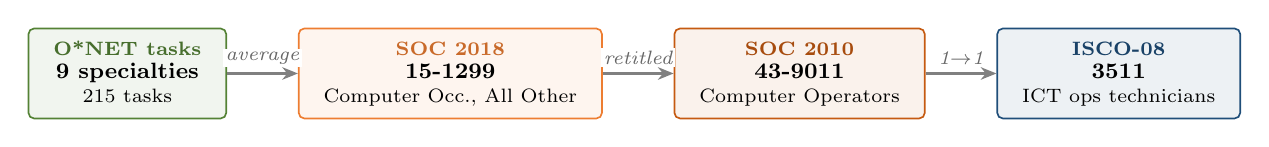
\begin{tikzpicture}[node distance=0.9cm and 0.9cm]
  \node[codebox=cTASK] (task) {\cbox{cTASK}{O*NET tasks}{9 specialties}{215 tasks}};
  \node[codebox=cSOC18, right=of task] (soc18) {\cbox{cSOC18}{SOC 2018}{15-1299}{Computer Occ., All Other}};
  \node[codebox=cSOC10, right=of soc18] (soc10) {\cbox{cSOC10}{SOC 2010}{43-9011}{Computer Operators}};
  \node[codebox=cSTYRK, right=of soc10] (isco) {\cbox{cSTYRK}{ISCO-08}{3511}{ICT ops technicians}};

  \draw[chain] (task) -- node[arrowlabel]{average} (soc18);
  \draw[chain] (soc18) -- node[arrowlabel]{retitled} (soc10);
  \draw[chain] (soc10) -- node[arrowlabel]{1$\to$1} (isco);
\end{tikzpicture}

\vspace{0.6em}
\footnotesize
The SOC 2010 → 2018 re-coding turned ``Computer Operators'' into the catch-all ``Computer Occupations, All Other'' (15-1299), which contains nine sub-specialties. The Eloundou et al.\ pipeline averages those nine specialty means; tasks are not aggregated directly.
\end{frame}

% specialty table
\begin{frame}{Specialty-level scoring: Computer Occupations, All Other (15-1299)}
\centering\small
\setlength{\tabcolsep}{6pt}
\renewcommand{\arraystretch}{1.05}
\begin{tabular}{lp{5.5cm}cc}
\toprule
O*NET-SOC & Title & N tasks & specialty $\beta$ \\
\midrule
15-1299.01 & Web Administrators                            & 23 & 0.913 \\
15-1299.02 & Geographic Information Systems Technologists  & 27 & 0.593 \\
15-1299.03 & Document Management Specialists               & 18 & 0.611 \\
15-1299.04 & Penetration Testers                           & 22 & 0.795 \\
15-1299.05 & Information Security Engineers                & 20 & 0.675 \\
15-1299.06 & Digital Forensics Analysts                    & 20 & 0.725 \\
15-1299.07 & Blockchain Engineers                          & 17 & 0.971 \\
15-1299.08 & Computer Systems Engineers/Architects         & 28 & 0.768 \\
15-1299.09 & Information Technology Project Managers       & 21 & 0.571 \\
\midrule
\multicolumn{4}{l}{\textbf{SOC $\beta$ (mean of 9 specialties): \;0.736 (Q5)}} \\
\bottomrule
\end{tabular}

\vspace{0.7em}
\footnotesize
The 9 specialties carry exposure scores ranging from 0.57 to 0.97. The Norwegian title ``Driftsteknikere, IKT'' best matches Web Administrators or Computer Systems Engineers/Architects; the score that lands on STYRK 3511 is an average over a wider set of computing roles.
\end{frame}

% Many-to-one mapping example (split out of eloundou.tex so the worked
% examples for the five additional one-to-one occupations can be inserted
% in between).

\begin{frame}{Worked example: many-to-one mapping}
\centering
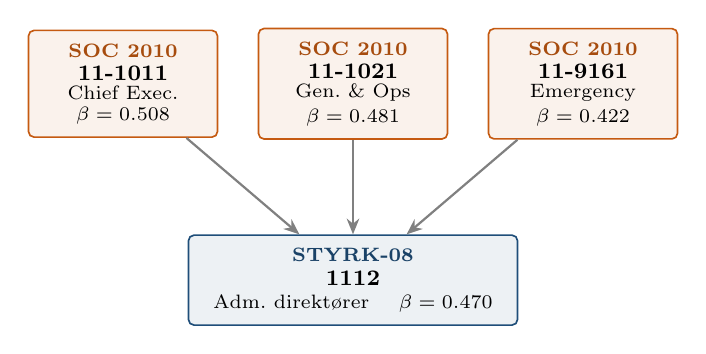
\begin{tikzpicture}[node distance=0.4cm and 0.5cm]
  \node[codebox=cSOC10] (a) {\cbox{cSOC10}{SOC 2010}{11-1011}{\shortstack{Chief Exec. \\ $\beta=0.508$}}};
  \node[codebox=cSOC10, right=of a] (b) {\cbox{cSOC10}{SOC 2010}{11-1021}{\shortstack{Gen.\ \& Ops \\ $\beta=0.481$}}};
  \node[codebox=cSOC10, right=of b] (c) {\cbox{cSOC10}{SOC 2010}{11-9161}{\shortstack{Emergency \\ $\beta=0.422$}}};

  \node[codebox=cSTYRK, below=1.2cm of b, minimum width=3.5cm] (s) {\cbox{cSTYRK}{STYRK-08}{1112}{Adm.\ direktører \quad \textbf{$\beta=0.470$}}};

  \draw[chain] (a) -- (s);
  \draw[chain] (b) -- (s);
  \draw[chain] (c) -- (s);
\end{tikzpicture}

\vspace{0.4em}
\footnotesize
\begin{itemize}\setlength{\itemsep}{1pt}
  \item Three SOC 2010 codes map to ISCO 1112 in the BLS crosswalk
  \item STYRK $\beta$ is the unweighted mean of contributing SOC-level $\beta$
  \item $57.7\%$ of Eloundou et al.\ STYRK codes have at least one contributor flagged as a partial match in the BLS file
\end{itemize}
\end{frame}

% O*NET data structure: background for the four measures

\begin{frame}{O*NET: the US occupation database underneath three of the four measures}
\begin{itemize}\setlength{\itemsep}{6pt}
  \item Maintained by the US Department of Labor; covers $\sim$1{,}000 occupations on SOC~2018 codes (O*NET-SOC 2019 taxonomy)
  \item Each occupation has structured content:
  \begin{itemize}
    \item \textbf{Tasks:} discrete activities ($\sim 19{,}000$ across all occupations; Pharmacists: 21 tasks, e.g.\ ``review prescriptions for accuracy''). Tagged \emph{Core} or \emph{Supplemental}; no numerical weight.
    \item \textbf{Abilities:} 52 underlying attributes (e.g.\ Deductive Reasoning, Manual Dexterity). Scored on prevalence and importance per occupation.
    \item Also: skills, knowledge, work activities, work context (not used by the four measures here).
  \end{itemize}
  \item Eloundou et al.\ and Handa operate on \textbf{tasks}; Felten operates on \textbf{abilities}; Anthropic 2026 operates at the occupation level.
\end{itemize}
\end{frame}



\end{document}
